\documentclass[a4paper,oneside,11pt]{report}

\usepackage{mystyle}

\begin{document}

\pagestyle{empty}
\pagenumbering{alph}
\documentclass{standalone}
\usepackage{standalone}

\begin{document}

\begin{titlepage}
\begin{center}

    {\huge \bf Shahjalal University of Science and Technology}\\
    {\LARGE \bf Department of Computing Science and Engineering}

    \vfill
    \begin{figure}[h]
    \centering
    
\includegraphics[scale=0.6]{./img/varsityLogo}
    \end{figure}


    \vfill 
    {\LARGE \bf Automated Bangla License Plate Recognition}\\      
    \begin{multicols}{2}
    \textsc{\Large Md. Al-amin Nowshad}\\
    Reg. No.: 2012331059\\ $4^{th}$ year, $1^{st}$ Semester\\
    \textsc{\Large Sudipto Chandra Das} \\
    Reg. No.: 2012331019\\ $4^{th}$ year, $1^{st}$ Semester
    \end{multicols}

	\vfill
    Department of Computer Science and Engineering\\
    
	\vfill
    {\bf Supervisor}\\
    \textsc{\Large Md. Jahirul Islam} \\
    Professor\\ 
    Department of Computer Science and Engineering\\
    
    \vfill
	\today
        
\newpage
	
    \vspace{0.5cm}
    {\Large \bf Automated Bangla License Plate Recognition}
    \begin{figure}[h]
	\centering
	
\includegraphics[scale=0.6]{./img/varsityLogo}
	\end{figure}\\
    
    \vspace{0.5cm}
	A Thesis submitted to the \\
    {\large Department of Computing Science and Engineering}\\
    {\Large Shahjalal University of Science and Technology}\\
    Sylhet - 3114, Bangladesh
	
	in partial fulfillment of the requirements for the degree of \\
        
    {\Large Bachelor of Science in Computer Science and Engineering}\\
    
    \vfill {\LARGE By}\\
    \begin{multicols}{2}
    \textsc{\Large Md. Al-amin Nowshad }\\
    Reg. No.: 2012331059\\ $4^{th}$ year, $1^{st}$ Semester\\
    \textsc{\Large Sudipto Chandra Das} \\
    Reg. No.: 2012331019\\ $4^{th}$ year, $1^{st}$ Semester\\ 
	\end{multicols}
	
    \vfill Department of Computer Science and Engineering
    \vfill
    {\bf Supervisor}\\
    \textsc{\Large Md. Jahirul Islam} \\
    Professor\\ 
	Department of Computer Science and Engineering\\
    
    \vfill
    \today
    
\end{center}

\newpage

\begin{center}
	\textbf{\huge Recommendation Letter from Thesis Supervisor}
\end{center}
	
    \vspace{0.5cm}
    
    \noindent
	The thesis\\
    entitled "{Automated Bangla License Plate Recognition}"\\
    submitted by the students
	\begin{enumerate}
		\item Md. Al-amin Nowshad
		\item Sudipto Chandra Das
	\end{enumerate}
	is a record of research work carried out under my supervision and I, hereby, approve that the report be submitted in partial fulfillment of the requirements for the award of their Bachelor Degrees.\\
	
    \vspace{4.0cm}
	
    \noindent
	Signature of the Supervisor: \\
	Name of the Supervisor: \textsc{\large Md. Jahirul Islam}\\% adds space between the two sets of signatures
	Date: \today
				
\newpage

\begin{center}
	\textbf{\huge Certificate of Acceptance of the Thesis} \\
\end{center}
	
    \vspace{0.5cm}
    
	\noindent
	The thesis\\
	entitled "{Automated Bangla License Plate Recognition}"\\
	submitted by the students
	\begin{enumerate}
		\item Md. Al-amin Nowshad
		\item Sudipto Chandra Das
	\end{enumerate}	
    on \today
    \noindent
	is, hereby, accepted as the partial fulfillment of the requirements for the award of their Bachelor Degrees.
				
    \vspace{4.0cm}
				
\begin{multicols}{3}	
	\begin{flushleft}
		\hrulefill \\
        \centering
		Head of the Dept.
	\end{flushleft}
	
    \begin{flushleft}
		\hrulefill \\
        \centering
		Chairman,\\ 
        Exam Committee.
	\end{flushleft}				
	
    \begin{flushleft}
		\hrulefill \\
        \centering
		Supervisor
	\end{flushleft}    
\end{multicols}
    

\end{titlepage}
\end{document}

\pagestyle{plain}

\clearpage
\pagenumbering{Roman}
\addcontentsline{toc}{section}{Abstract}
\documentclass{standalone}
\usepackage{standalone}

\begin{document}
\chapter*{Abstract}

\makebox[\textwidth]{\it This is primary abstract. It may change in future.}\\

Automated license plate recognition is important in many contexts like- security and law enforcement, monitoring vehicles, automated parking control. To enable these automated services in Bangladesh we are proposing an efficient method in this paper. The task of recognizing vehicle number plate consists of three stage: plate detection, character segmentation and character recognition. We reviewed several methods for each stage, and choose the best one. The main objective of this research is to gain high accuracy in an efficient manner, keeping into consideration the facts of lighting conditions, vehicle motion, noisy plates, segmented words. Our primary target is to recognize the standard bangla license plates. But we also tested our methods on non-standard license plates.
%
For standard license plate we have gained {\bf XX\%} accuracy in plate detection, {\bf XX\%} in character segmentation and {\bf XX\%} in recognition, resulting in {\bf XX\%} accuracy overall.


\vspace{1.0cm}
%\clearpage

\paragraph*{Keywords:} Automated License Plate Recognition (ALPR), Bangla Number Plate, Image Enhancement, Number Plate Detection, Bangla Character Segmentation,  Bangla Character Recognition. 

\end{document}


\clearpage
\addcontentsline{toc}{section}{Acknowledgement}
\documentclass{standalone}
\usepackage{standalone}

\begin{document}
\chapter*{Acknowledgements}
We would like to thank the Department of Computer Science and Engineering, Shahjalal University of Science and
Technology, Sylhet 3114, Bangladesh, for supporting this research. We are very thankful to our honorable teacher Prof. Md. Jahirul Islam for his outstanding directions and help.  

We are also grateful to anonymous authors of previous works.
\end{document}


\clearpage
\addcontentsline{toc}{section}{Dedication}
\documentclass{standalone}
\usepackage{standalone}

\begin{document}
\chapter*{Dedication}
We would like to dedicate our research to our parents. We are also grateful to anonymous authors of
previous works for their co-operation and support.
\end{document}


\clearpage
\addcontentsline{toc}{section}{Table of Contents}
\tableofcontents

\clearpage
\addcontentsline{toc}{section}{\listtablename}
\listoftables

\clearpage
\addcontentsline{toc}{section}{\listfigurename}
\listoffigures


\clearpage
This is a citation example\: \cite{AEBCAM_LPD}. Very easy.
\clearpage


\clearpage
\pagenumbering{arabic}
\documentclass{standalone}
\usepackage{standalone}

\begin{document}
\chapter{Introduction}
In the field of Image processing and computer vision license plate recognition is an well established title. This thesis tries to implement this established title for license plates written in Bengali language with the purpose of making the previous system well organized and more efficient.  

Automated license plate recognition systems are available for commercial use with great cost for other languages used in mainly fields like - traffic history check, security maintenance, parking, etc. 

\section{Objectives}
The main objective of this thesis is to find out an efficient way to implement the ALPR system for Bengali digital license plates. The main objective is divided into sub objectives like - turning the system into a full working application which should be open sourced and organized for further use. 

\section{Challenges}
For fulfilling objectives there are few challenges to conquer. These challenges are -
	\begin{enumerate}
		\item reviewing and finding lacking of previous systems
		\item implement multiple systems to get a better review and future planning
        \item gather license plate image dataset
        \item preprocessing dataset properly and handling different cases
        \item implementing two different main sections - license place extraction and character recognition properly for Bengali language.
        \item comparing and performance enhancement of the developed system.
	\end{enumerate}
    
\section{Motivation}
As there is no established ALPR system in Bangladesh although few thesis related to this field already been done, it is time to make something properly usable and complete. As the main thought of making a real world effect, it is needed to find and implement a way to make a working Bengali ALPR system.

\section{Approaches}
Primarily the approach of this thesis has to be able to make a system working with the limited resources with low cost. Industrial ALPR systems are far more expensive and takes a huge amount of time, money, data which is not affordable in the scope if this thesis. So, ordinary camera images are used as dataset with minimal resolution.

The license plate extraction part is done trying few traditional techniques and also with some out of the box techniques which will be described in the later chapters. And further iterations of tuning the current system will be made in the next section of time frame for this thesis work.

Optical character recognition is the second part of this research work. This is itself a big field which includes past researches for Bengali language. Most of those researches are not of good quality to implement directly in this thesis. But, the datasets can be re-used to for training purposes. So, two approaches are under consideration- using Google's Tesseract OCR and using previous works for Bangla OCR. Both will be tried in the next part of this thesis work. 

\section{Thesis Structure}
The structure of this thesis report is mainly divided into three parts - introductory discussion including history and other background knowledges related to this field, the technical implementation and review, result analysis and conclusion.


\end{document} 		% includes background

\documentclass{standalone}
\usepackage{standalone}

\begin{document}
\chapter{Background Study}

\section{Historical View}
As far as we know that ANPR system was first invented in 1976. It was done by the Police Scientific Development Branch in the UK. Industrial usage begun in 1979. But ANPR got more known in the 1990's for their cheap implementation from the previous costly systems. The first ANPR dataset was made in early 2000s. This system was used to solve a murder occurred in November 2005, in Bradford, UK, to locate and find the culprits behind the killing of Sharon Beshenivsky.

From that point forward tag acknowledgment has advanced and been utilized by police and different associations for various purposes and has turned out to be less expensive and speedier, yet not sufficiently shoddy for private utilize. In the following areas, a portion of the current techniques in the zone of tag location and acknowledgment will be talked about.

\section{Literature Review}
The first task was to find the problem domain to work on. The next task was to make literature reviews for our work plan and also for ensuring that we are not doing something again or worse. We've found few papers related to ALPR for Bengali languages and many more in different languages. Finally, we did select 24 papers to read and review for our thesis work. We've written 7 review papers those seemed close to our topic. From those papers and reviews we've managed to find and understand our particular domain of work which will be described in the later parts.
\end{document} 	% includes intro of literature review
\section{Standard Bangla license plate}
\subsection{Vehicle types}
Vehicles are of different types in Bangladesh. As a result license plates don't stay at the same place for each vehicle.
Vehicles considered in this thesis work are - private car, bus, cng auto-rickshaw, truck. Though there were no previous format and standardization of the license plate in the past, currently government has enforced digital license plate for all vehicles which makes it a new case to handle and less error prone than the previous systems.

\subsection{Structure of the plate}
The digital Bengali license plate is normally written in two lines.

    \begin{figure}[ht]
    \centering
    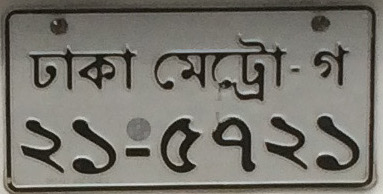
\includegraphics[scale=0.8]{./img/sample_plate}
    \caption{Example of a digital license plate in Bangla}
	\label{fig:EX}
    \end{figure}

\par
As the example given the line on the top written in Bangla and the bottom line has all digits in Bangla.    

\subsection{Parts of plate number}
The top line got two parts. First part before the '-' denotes the city of the car license and then the second part denotes the series it is in.

The bottom line is the number of the license assigned to the particular vehicle by the licensing rules and regulation of Bangladesh Road Transport Authority.

	\begin{figure}[ht]
    \centering
    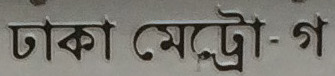
\includegraphics[scale=0.8]{./img/up}
    \caption{upper portion of license plate}
	\label{fig:UP}
    
    
\includegraphics[scale=0.8]{./img/down}
    \caption{bottom part of license plate}
	\label{fig:DOWN}
    
    \end{figure} 
\subsection{Plate fonts}
Digital license plate is offering verified fonts, but in Bangladesh those rules are not strictly followed by all vehicle owners. Also the current dataset doesn't have any universal font. So, the fonts can be different but easily understandable for this thesis work.

\section{Related Works}
The rest of the chapter will discuss some of the previous works related to license plate recognition.The whole task is divided into five main steps: Preprocessing, Feature analysis, Region analysis, Character segmentation, Recognition.
	
    \begin{figure}[ht]
    \centering
    \includegraphics[scale=1.0]{./img/steps}
    \caption{Steps of ALPR system}
	\label{fig:STEPS}
    \end{figure} 
    
These steps are going to be discussed briefly in this chapter.
\clearpage
\documentclass{standalone}
\usepackage{standalone}

\begin{document}
\section{Preprocessing}
Preprocessing techniques are used to get a better performance in the next sections. This is one of the key task after image acquisition. It ensures good data input for the main parts of the license plate detection and recognition system.

Most common approach is done in two steps. The image is converted to a gray scale image format to the next steps (Waterhouse-2006) \cite{waterhouse-2006}. Then, any additional noise is reduced from the image with different types of algorithms in different cases. Most common techniques for reducing noise from input image are the Median filter(Songke and Yixian-2011)
and Gaussian filter(Sedighi and Vafadust 2011). Contrast enhancement is an additional technique followed by many researchers(Abolghasemi and Ahmadyfard - 2009) in this pre-processing part.

\end{document}
\section{Feature Analysis}

For detecting the license plate, feature analysis must be done after an image is preprocessed properly.
Checking the edges for detecting any rectangle shaped area is the most common technique for feature analysis.
To detect the plate boundary, some researchers use horizontal lines and others look for vertical lines.
Edge detection is commonly done with Canny (Kong, Liu, Lu, and Zhou-2005) and Sobel edge detection (Jiao, Ye, and Huang 2009).
As foe some exception some researches do not use edge detection, but try to find high contrast area (Huang, Chang, Chen, and Sandnes-2008). The theory behind this technique is - plates generally have higher contrast area than other parts of the image.
\section{Region Analysis}

When the feature analysis is done, it is possible that several regions of the image can be candidates for the license plate portion. For solving this problem some filtering is needed to lower the number of candidates by analyzing and removing them. A very common technique to do the task is to consider features of the bounding rectangle of candidate region. For example we can consider - aspect ratio, size width, height and location for candidate filtering. For example, calculating the rectangles features for determining the license plate probable region is a common trick (Yoon,
Lee, and Lee - 2009). Also, Abolghasemi and Ahmadyfard (2009), Tsai, Wu,
Hsieh, and Chen (2009) and Kong et al. (2005) used some geometrical features of the candidate
regions to detect the actual plate region. Following this with
further addition of techniques Gazcón, Chesñevar, and Castro (2012) proposed that if the region can be divided into well defined siz sub sections then it is the license plate region. Other researches like Hung and Hsieh (2010) used geometrical features technique
with a more or less the same technique by considering characters into
of the number plate while filtering the candidate regions. A slightly different approach for determining the license plate region was proposed by Chen, Chen, Huang, and Wang
(2011) by using the high density edges followed by horizontal projection.

\section{Character Segmentation}

For recognition of the characters sometimes it is needed to segment them before sending them to the recognition system. Different research used different techniques for this part of work.

Using histogram to segment the characters is a common trick first used by Songke and Yixian (2011) and Huang et al. (2008). The technique was to use the accumulation or summation of the vertical and horizontal projections. Connected-component labeling algorithm can be used for the purpose of character segmentation which was used by Yoon et al. (2009) and Maglad (2012). The algorithm acts in two steps. Detection of the connected characters those are in black while the background is white. Then labeling those character blobs with bounding box. This technique was implemented by Liaqat (2011) using two algorithms, Canny for detecting the edges then contour finding algorithm to find the connected edges. Labeling and segmentation can be done using other methods. Next recognition step used many of the information gained in this step. All these information can be passed to a method for recognizing characters. Tsai et al. (2009) tried further judgement of this step to ensure that the selected characters makes the actual license plate, not some other part of the image. The conditions to pass this test were that the width, and height of character rectangles must be similar, character density should be in a range, and the width must be less than the height.
\section{Character Recignition}

For licesnse plate recognition there are few ways to complete the character recigntion part. The most common technique can be divided into two steps. At first, the characters from the previous step are provided to a recognition engine that can be coded or used as a package. For example, Open source Tesseract OCR is a great choice for character recognition engine. It generates text output from the given image of characters if it is well trained. In the second approach is to implement bespoke recognition methods. For each individual character, features are computed. For recognizing the characters, OCR system will extract features first, then compare them against patterns that have been implemented earlier (Juntanasub and Sureerattanan - 2005). Alginahi (2011) tried  to extract 88 features for each character following the same approach, then compared these features with previously extracted features. Songke and Yixian (2011) used histogram to extract characters and template matching for recognition. Later when the neural network techniques got famous, Ghosh, Sharma, Islam, Biswas, and Akter - 2011 used them for character recognition. The module is trained first and then used for recognizing characters using the previously given taining feature dataset.
\section{Comparisons}

The accuracy of license plate recognition system can be described in three parts - license plate detection, character recogntion, overall accuracy. The table below gives an overview related to the approach and problems of some previous research work-

\begin{table}[]
	\centering
	\caption{Comparison Table}
	\label{tab:error5}
	\begin{tabular}{|c|c|c|c|}
		\hline
		\begin{tabular}[c]{@{}c@{}}Author and year\end{tabular} & \begin{tabular}[c]{@{}c@{}}Detection (\%)\end{tabular} & 
		    \begin{tabular}[c]{@{}c@{}}Recogntion (\%)\end{tabular} & 
		    \begin{tabular}[c]{@{}c@{}}Overall (\%)\end{tabular} \\ \hline
		    
		BWA-MEM & 88.4 & 11.6 \\ \hline
		NanoBLAST & 86.55 & 13.45 \\ \hline
		NanoMapper & 97.42 & 2.58 \\ \hline
	\end{tabular}
\end{table}

\section{Summary}


Review of previous works shows that the edge detection approach can be used effectively to find the license plate region. Geometrical feature analysis is an appropriate approach for this. Some researches used their own recogntion system, others used OCR engines like - teserract. Some parts of all these research can be used further in this work, others are of no use for future work.



\documentclass{standalone}
\usepackage{standalone}

\begin{document}

\chapter{Methodology}
This chapter describes our process to detect license plate given an input image, and separation of the individual numbers and character sequence from detected license plate. The input image may come from variety of sources. We have put on a validation method to detect if there is actually a license plate in the input image.

  \documentclass{standalone}
\usepackage{standalone}

\begin{document}

\section{Implementation}
We implemented our solution using {\it Python-3.x} using the {\it OpenCV-3} and {\it Numpy} libraries from Anaconda repository. 
The {\it OpenCV} library provides an extensive collection of image processing functions and techniques which proved very helpful in our implementation. 
{\it Numpy} has been used the most to manipulating 2D arrays, and in our design of Multilayer Perceptron model for recognizing characters.

For testing and analysis we used a separate implementation. In this implementation, we divided entire tasks into sequence of {\bf stages}. This {\it stages} act like individual modules. For example, a stage for Gaussian filter will only apply Gaussian filter to a set of input image and save the output to another folder to make it useful as input for later stages. This approach on testing proved to be quite useful and saved a lot of time during our research.

The installation and testing process of our implementation in provided in Appendix \ref{chap:install}.

\end{document}
  \documentclass{standalone}
\usepackage{standalone}

\begin{document}

\section{Overview}
We separate our process into several stages. Each stages contains several steps in it. An overview of all stags in our process is shown in Figure \ref{fig:ProcessOverview}. The process will be described in more details in the following sections.

\begin{figure} 
	\centering
	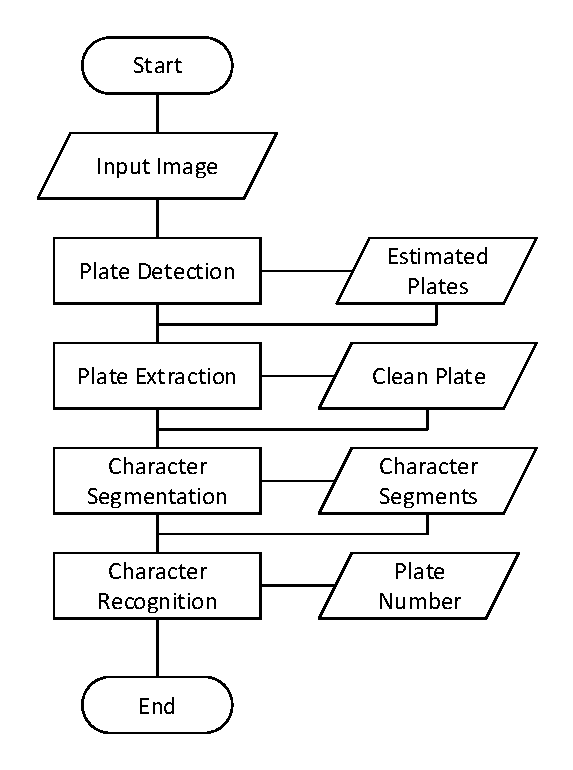
\includegraphics[width=0.8\linewidth]{./img/plots/overview}
	\caption{An overview of the plate detection procedure.} 
	\label{fig:ProcessOverview}
\end{figure}

\begin{description}
\item [Input Image] is a 24-bit colored image with red, green and blue channels.
\item [Preprocessing] stage applies several operations on input image to convert it into an image suitable for feature analysis for later stages. In our case, it also outputs general location of the plate.
\item [Plate Detection] analyses all plate like locations, and extract plates from them. Also it cleans the plate for segmentation.
\item [Segmentation] step is for splitting the characters from the plate. It is done so that the characters can be recognized by the OCR.
\item [Plate recognition] uses an OCR system to recognize individual characters and text images.
\end{description}

\end{document}

\section{Preprocessing}
This stage contains a sequence of steps that enhance the plate like regions of an image and output an image that can be used directly for the next stage - plate detection.

  \documentclass{standalone}
\usepackage{standalone}

\begin{document}
\subsection{Rescale}
By minimizing the size of an image we can reduce processing time dramatically. But reducing image may result in loss of information. From reviews, we decided to use the dimension: $640 \times 480$. We re-scale the input image into this dimension at first step. Figure \ref{fig:RescaledSample} shows a sample image.

\begin{figure}
	\centering
	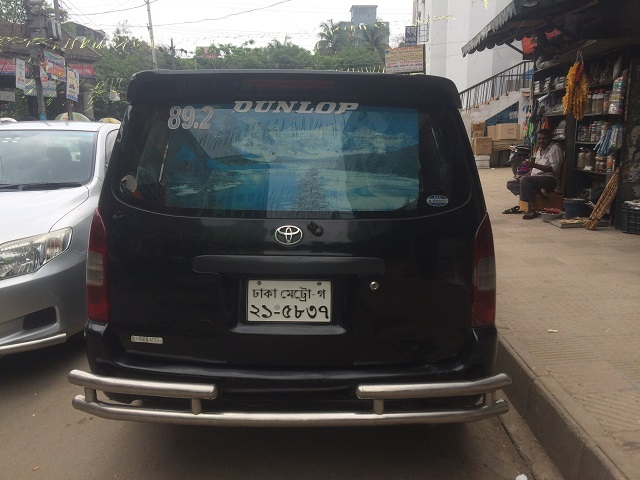
\includegraphics[width=.8\linewidth]{./img/sample/stage0.jpg}
	\caption{A sample input image (rescaled)}
	\label{fig:RescaledSample}
\end{figure}

\end{document}
  \documentclass{standalone}
\usepackage{standalone}

\begin{document}
\subsection{Gray Scale Conversion}
From the 24-bit color value of each pixels $(i, j)$ of the input image, we split the $R$, $G$, $B$ components . Then, 8-bit gray value is calculated using the following formula:
\begin{equation}
gray(i,j) = 0.59 * R(i,j) + 0.30 * G(i,j) + 0.11 * B(i, j)
\end{equation}

\begin{figure}
	\centering
	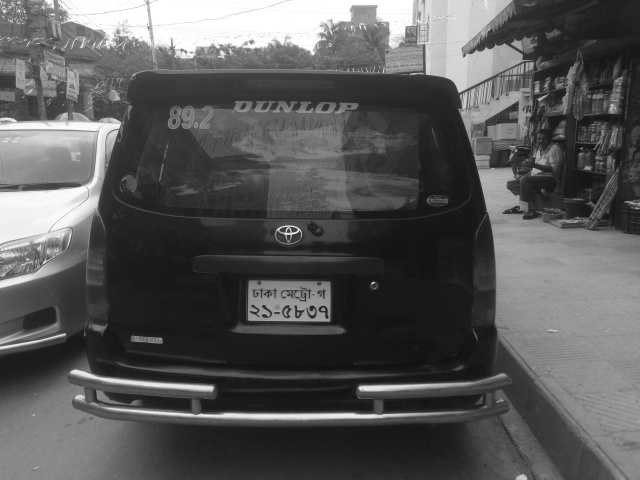
\includegraphics[width=.8\linewidth]{./img/sample/stage1.jpg}
	\caption{A sample gray-scale image} 
	 \label{fig:GraySample}
\end{figure}

\end{document}
  \documentclass{standalone}
\usepackage{standalone}

\begin{document}

\subsection{Vertical Edge Density}
The vertical {\it Sobel operator} (Equation \ref{eq:Sobel}) is used to calculated the edge density. 
\begin{equation} \label{eq:Sobel}
h =
  \begin{bmatrix}
    -1 & 0 & 1\\
    -2 & 0 & 2\\
    -1 & 0 & 1
  \end{bmatrix} 
\end{equation}

Which we could obtain by using $sobel$ function from OpenCV library:
\begin{lstlisting}[language=Python]
sobel = cv2.Sobel(img, cv2.CV_8UC1, 1, 0, ksize=3)
\end{lstlisting}

Next, we applied a low threshold value to the gradient image. In this case, we used an adaptive threshold technique called {\it Otsu’s Binarization} using an offset value of $85$, which we obtained empirically. Result is shown in Figure \ref{fig:SobelSample}

\begin{figure}
	\centering
	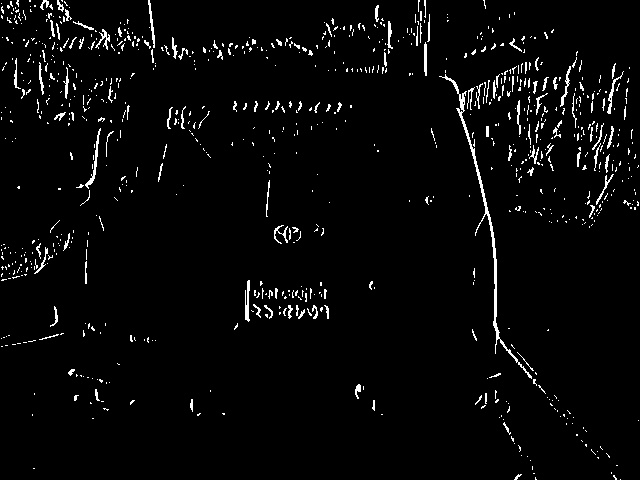
\includegraphics[width=.8\linewidth]{./img/sample/stage2.jpg}
	\caption{After applying Sobel Operator} 
	\label{fig:SobelSample}
\end{figure}

\end{document}
  \documentclass{standalone}
\usepackage{standalone}

\begin{document}

\subsection{Gaussian Filter}
In this step, 2D Gaussian filter is applied to the gradient image from previous step. We used a Gaussian kernel of size $60 \times 60$. To calculate the kernel the formula in Equation \ref{eq:GaussFilter} is used. Figure \ref{fig:GaussianFilterPlot} shows a plot of this filter.
\begin{equation} \label{eq:GaussFilter}
g(i, j) = \dfrac{\alpha}{2\pi\sigma^2} \cdot e^{\frac{i^2 + j^2}{2\sigma^2}}
\end{equation}

\begin{figure} 
	\centering
	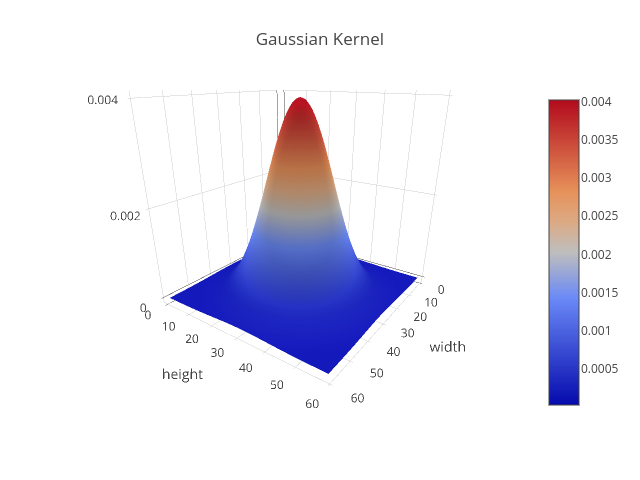
\includegraphics[width=.8\linewidth]{./img/plot/gauss.jpg}
	\caption{Applied the Gaussian Blur} 
	\label{fig:GaussianFilterPlot}
\end{figure}

Here, the blur coefficient $\alpha$ and the $\sigma$ are set empirically. We used $filter2D$ function to apply convolution of on the gradient image
\begin{lstlisting}[language=Python]
gauss = cv2.filter2D(sobel, cv2.CV_64F, kernel)
\end{lstlisting}

As a result we get a nicely blurred image (Figure \ref{fig:GaussianSample}).
\begin{figure} 
	\centering
	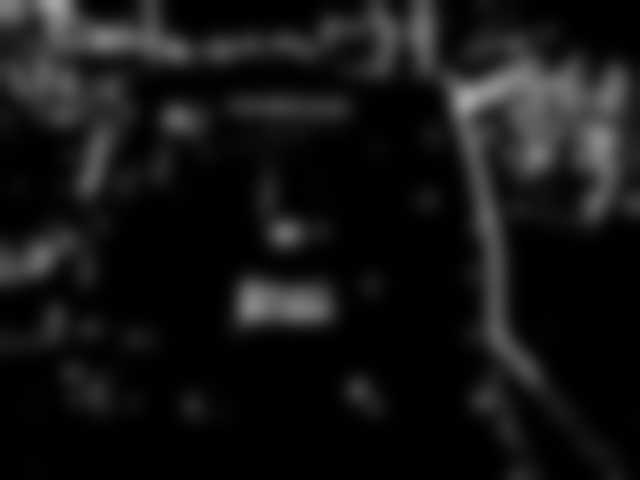
\includegraphics[width=.8\linewidth]{./img/sample/stage3.jpg}
	\caption{Applied the Gaussian Blur} 
	\label{fig:GaussianSample}
\end{figure}


\end{document}
  \documentclass{standalone}
\usepackage{standalone}

\begin{document}
\subsection{Image Enhancement}
We modified the enhancement techniques described in \cite{Abolghasemi2009} and \cite{zheng2005efficient} followed by \cite{joarder2012bangla}. We used the Gaussian image to increase the contrast of the image around plate like regions. The formula used is shown in Equation \ref{eq:Enhancement}.

\begin{equation} \label{eq:Enhancement}
I' = f(\rho W_g) (I - \bar{I}) + \bar{I}
\end{equation}

In the equation \ref{eq:Enhancement},\\
$\bar{I}$ = the mean intensity. \\
$I$ = the intensity of the original image. \\
$I'$ = the new enhanced image. \\
$W_g$ = normalized Gaussian image. \\ 
$\rho W$ = the standard deviation of Gaussian image, and \\
$f$ = the weighting function defined in Equation \ref{eq:WeightFunction}.
\begin{equation} \label{eq:WeightFunction}
f(\rho W_g) = 
\begin{cases} 
	\dfrac{3}{ \dfrac{2}{0.3^2} ( \rho W_g - 0.3)^2 + 1 },
    	& \mbox{if } 0 \leq \rho W_g < 0.3  
     \\
    
    \dfrac{3}{ \dfrac{2}{(0.5 - 0.3)^2} ( \rho W_g - 0.3)^2 + 1 },
    	& \mbox{if } 0.3 \leq \rho W_g < 0.5  
     \\
        
    1	& \mbox{if } \rho W_g \geq 0
\end{cases}
\end{equation} 

Figure \ref{fig:WeightDistribution} shows the map of weight function from \ref{eq:WeightFunction}.
\begin{figure}
	\centering
	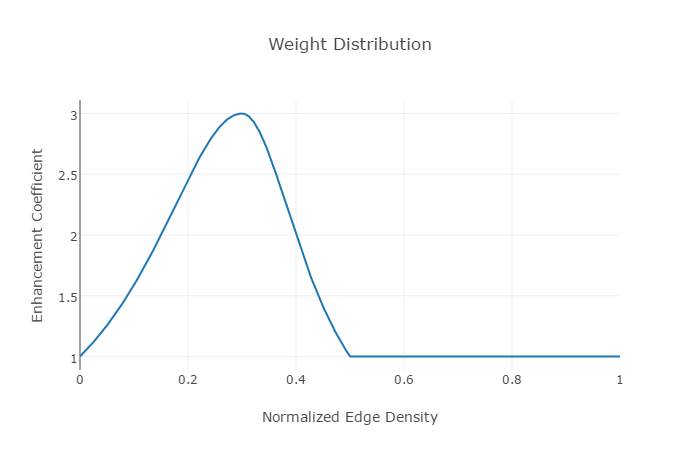
\includegraphics[width=.8\linewidth]{./img/plots/weight.png}
	\caption{Weight function against normalized edge density} 
	\label{fig:WeightDistribution}
\end{figure}

To increase the efficiency of the calculation the entire image is divided into $8 \times 8$ windows each having the size of $60 \times 80$. For each window we calculated weight and mean intensity using {\it Bilinear interpolation}. Also by using {\it numpy} library for matrix manipulation, we could dramatically decrease processing time.

Figure \ref{fig:EnhanceSample} shows the resulting image. The brightness of license plate area has significantly improved.
\begin{figure}
	\centering
	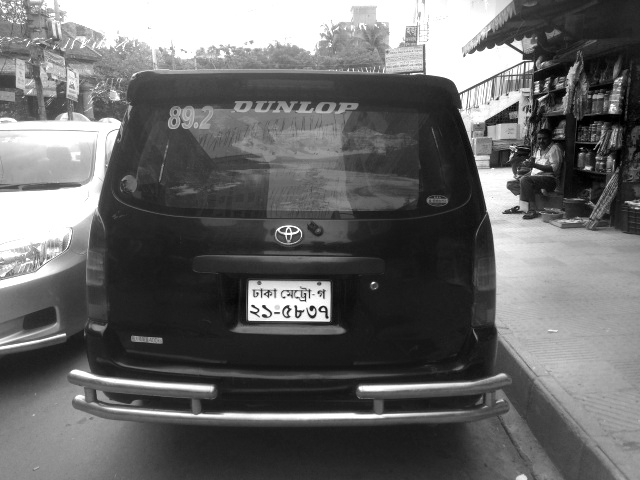
\includegraphics[width=.8\linewidth]{./img/sample/stage4.jpg}
	\caption{Enhanced Image} 
	\label{fig:EnhanceSample}
\end{figure}

\end{document}
  \documentclass{standalone}
\usepackage{standalone}

\begin{document}

\subsection{Matched Filter}
To detect the license plate, next step is to highlight plate like regions from the enhanced image. We used a mixture of Gaussian functions to emphasize the constancy of intensity values within plate-like regions along horizontal direction. Equation \ref{eq:MixtureModel} shows the mathematical model of this function. This function can properly model low edge densities above, below and at the middle of the car plate. 

\begin{equation} \label{eq:MixtureModel}
h(x, y) = 
\begin{cases} 
	A.exp \left(
    	\dfrac{ -\left(x - \dfrac{m}{6} \right)^2 }
        	{ 0.2 \sigma_x^2 } \right),                                      
    	& \mbox{for } 
        	0 \leq x \leq \dfrac{m}{3}, 
            0 \leq y \leq n     
    \\ \vspace{0.2cm}
    B.exp \left( 
    	\dfrac{ -\left(x - 
        			\left( \dfrac{m}{3} + \dfrac{m}{6} \right) 
                \right)^2 }
        	{ 2 \sigma_x^2 } \right),                
        & \mbox{for }
        	\dfrac{m}{3} \leq x \leq 2\dfrac{m}{6}, 
        	0 \leq y \leq n 
    \\ \vspace{0.2cm}
    A.exp \left( 
    	\dfrac{ -\left(x - 
        			\left( 2\dfrac{m}{3} + \dfrac{m}{6} \right) 
                \right)^2 }
        	{ 0.2 \sigma_x^2 } \right),
    	& \mbox{for } 
        	2\dfrac{m}{3} \leq x \leq m, 
            0 \leq y \leq n         
\end{cases}
\end{equation}


In the Equation \ref{eq:MixtureModel}, 
$A$ and $B$ are coefficients of the mixture model. These parameters are set empirically following the condition: $A > 0$ and $B < 0$. 
The symbol $\sigma_x$ is the variance of the main lobe toward x direction. 
Figure \ref{fig:MixtureModelPlot} shows a plot depicting this equation.
\begin{figure} 
	\centering
	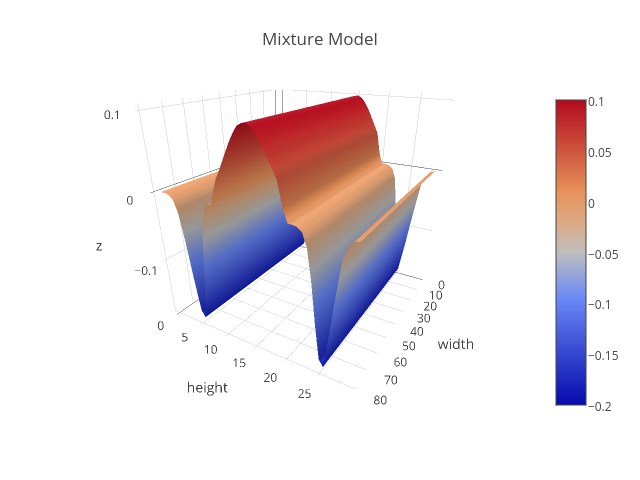
\includegraphics[width=.8\linewidth]{./img/plots/mixture.png}
	\caption{Gaussian Filter} 
	\label{fig:MixtureModelPlot}
\end{figure}

This filtering process provides a strong response at plate-like regions (Figure \ref{fig:OriginalMixtureModel}). The result is compared against a predefined threshold value, which is around $80\%$ of the maximum intensity. We call this process as smoothing, and the threshold value as {\it smoothing cutoff}.

\begin{figure}
\begin{subfigure}{.5\textwidth}
  \centering
  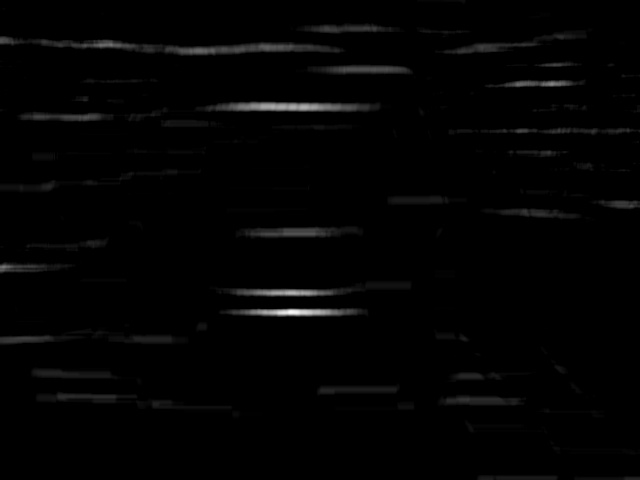
\includegraphics[width=.8\linewidth]{./img/sample/stage5-4.jpg}
  \caption{After applying the mixture model}
  \label{fig:OriginalMixtureModel}
\end{subfigure}
\begin{subfigure}{.5\textwidth}
  \centering
  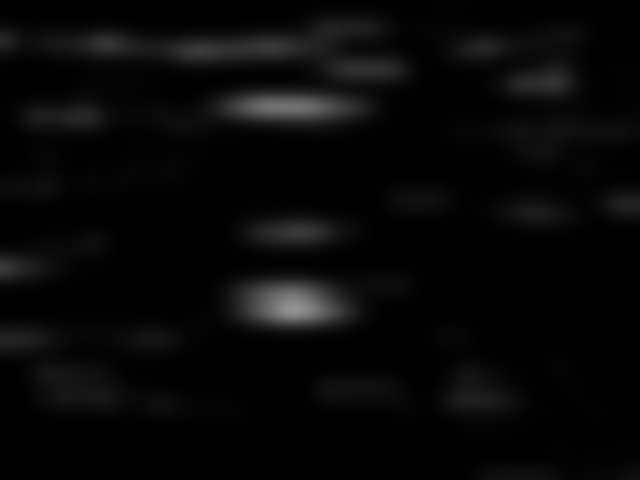
\includegraphics[width=.8\linewidth]{./img/sample/stage5-3.jpg}
  \caption{Gaussian blur on \ref{fig:OriginalMixtureModel}}
  \label{fig:BlurredMixtureModel}
\end{subfigure}
\begin{subfigure}{.5\textwidth}
  \centering
  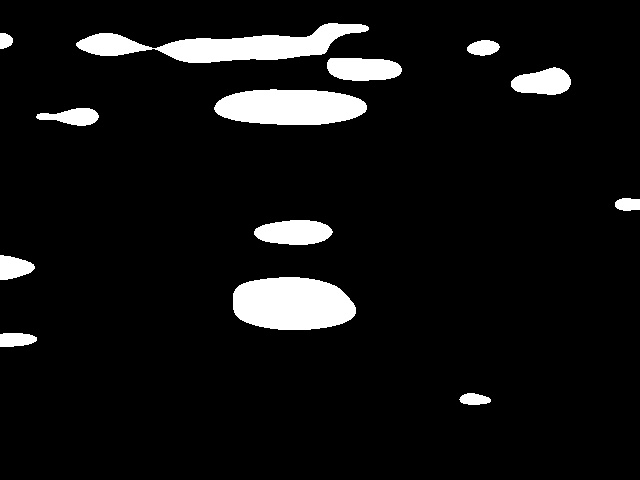
\includegraphics[width=.8\linewidth]{./img/sample/stage5-1.jpg}
  \caption{After applying adaptive threshold}
  \label{fig:ThresholdMixtureModel}
\end{subfigure}
\begin{subfigure}{.5\textwidth}
  \centering
  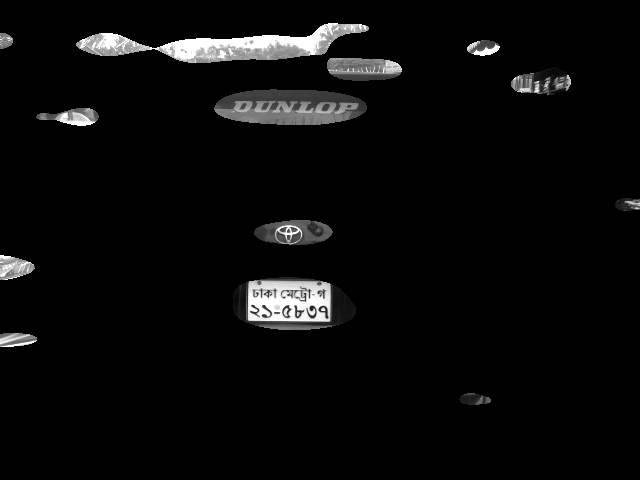
\includegraphics[width=.8\linewidth]{./img/sample/stage5-2.jpg}
  \caption{A see-through view of \ref{fig:ThresholdMixtureModel} with main image}
  \label{fig:GlassViewMixtureModel}
\end{subfigure}
\caption{Images after applying mixture model.}
\label{fig:MixtureModel}
\end{figure}


\end{document}
  \documentclass{standalone}
\usepackage{standalone}

\begin{document}
\subsection{Plate and regions extraction}
This step extracts the license plate and its bounding regions primarily. This does not detect actual license plate. But gives a close approximation to the location of the license plate. First we calculated all contours of the image calculated by mixture model. Next for each contours, we validated the bounding rectangle it is in. If the size of the bounding rectangle is valid, we extract the image of the area and region data. The extracted plates from the previous stage is shown in Figure \ref{fig:ExtractedPlates}.

\begin{figure}
\begin{subfigure}{.5\textwidth}
  \centering
  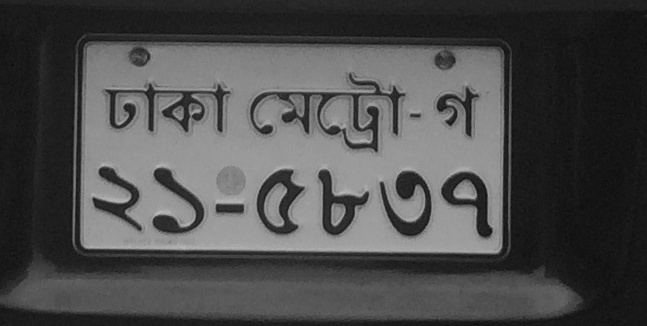
\includegraphics[width=.8\linewidth]{./img/sample/stage6-1.jpg}
  \caption{First estimation}
  \label{fig:FirstExtracted}
\end{subfigure}
\begin{subfigure}{.5\textwidth}
  \centering
  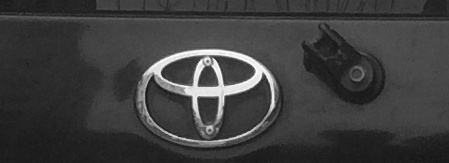
\includegraphics[width=.8\linewidth]{./img/sample/stage6-2.jpg}
  \caption{Second estimation}
  \label{fig:SecondExtracted}
\end{subfigure}
\begin{subfigure}{.5\textwidth}
  \centering
  
\includegraphics[width=.8\linewidth]{./img/sample/stage6-3.jpg}
  \caption{Third estimation}
  \label{fig:ThirdExtracted}
\end{subfigure}
\begin{subfigure}{.5\textwidth}
  \centering
  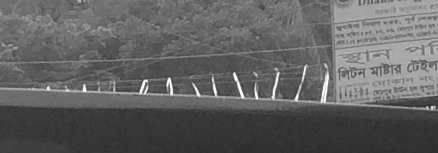
\includegraphics[width=.8\linewidth]{./img/sample/stage6-4.jpg}
  \caption{Fourth estimation}
  \label{fig:FourthExtracted}
\end{subfigure}
\caption{Estimated license plates.}
\label{fig:ExtractedPlates}
\end{figure}

\end{document}

\documentclass{standalone}
\usepackage{standalone}

\begin{document}

\section{Plate Detection}
This section describes the procedure to localize the license plate using the outputs from preprocessing stage. 

\begin{figure} 
	\centering    
	{\it put an image here }
	\caption{An overview of the plate detection procedure.} 
	\label{fig:DetectionMethod}
\end{figure}

\end{document}
  \documentclass{standalone}
\usepackage{standalone}

\begin{document}

\subsection{Edge Analysis}
Before detectining edges we first applied a threshold value to the estimated license plates (Figure \ref{fig:ThresholdCanny}).
\begin{figure}
\begin{subfigure}{.5\textwidth}
  \centering
  
\includegraphics[width=.8\linewidth]{./img/sample/stage7-1.jpg}
\end{subfigure}
\begin{subfigure}{.5\textwidth}
  \centering
  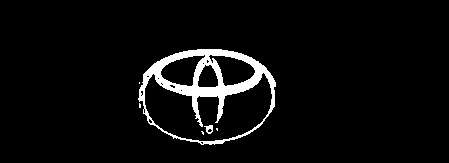
\includegraphics[width=.8\linewidth]{./img/sample/stage7-2.jpg}
\end{subfigure}
\begin{subfigure}{.5\textwidth}
  \centering
  
\includegraphics[width=.8\linewidth]{./img/sample/stage7-3.jpg}
\end{subfigure}
\begin{subfigure}{.5\textwidth}
  \centering
  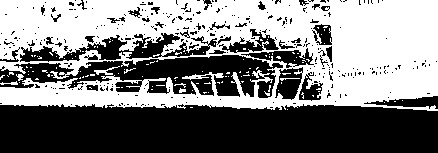
\includegraphics[width=.8\linewidth]{./img/sample/stage7-4.jpg}
\end{subfigure}
\caption{Applying threshold before Canny edge detection.}
\label{fig:ThresholdCanny}
\end{figure}

Canny Edge Detection is a popular edge detection algorithm. OpenCV has a direct function to it. We used the default function OpenCV provides to detect all edges of the localized estimated license plate image (Figure \ref{fig:CannyEdges}). 
\begin{lstlisting}[language=Python]
canny = cv2.Canny(img, 100, 200, L2gradient=True)
\end{lstlisting}

\begin{figure}
\begin{subfigure}{.5\textwidth}
  \centering
  
\includegraphics[width=.8\linewidth]{./img/sample/stage8-1.jpg}
  \caption{Edges of \ref{fig:FirstExtracted}}
\end{subfigure}
\begin{subfigure}{.5\textwidth}
  \centering
  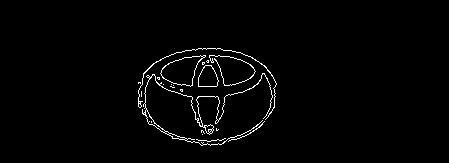
\includegraphics[width=.8\linewidth]{./img/sample/stage8-2.jpg}
  \caption{Edges of \ref{fig:FirstExtracted}}
\end{subfigure}
\begin{subfigure}{.5\textwidth}
  \centering
  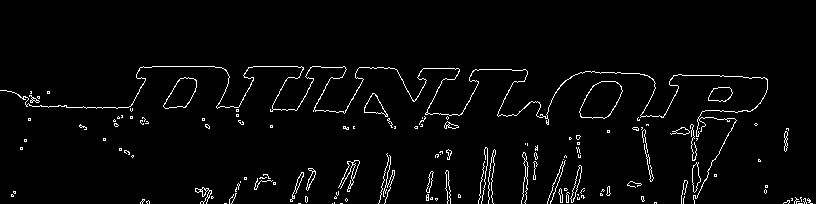
\includegraphics[width=.8\linewidth]{./img/sample/stage8-3.jpg}
  \caption{Edges of \ref{fig:FirstExtracted}}
\end{subfigure}
\begin{subfigure}{.5\textwidth}
  \centering
  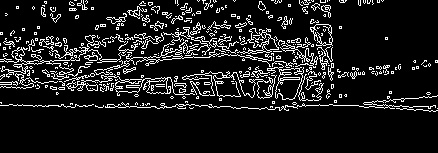
\includegraphics[width=.8\linewidth]{./img/sample/stage8-4.jpg}
  \caption{Edges of \ref{fig:FirstExtracted}}
\end{subfigure}
\caption{Result of Canny edge detecton algorithm.}
\label{fig:CannyEdges}
\end{figure}



\end{document}
  \documentclass{standalone}
\usepackage{standalone}

\begin{document}
\subsection{Contour Analysis}
Canny edge detection works perfectly for most cases and provides an easy to detect contours around plate borders \cite{alshahrani2013real}. After passing the canny image to the OpenCV's $findContours$ function, we get a set of contours. For each of these contours several parameters are checked according to \cite{alshahrani2013real} before selecting a contours as a possible plate. 

In this steps, some of the estimated candidate from previous stages fall out. In Figure \ref{fig:ContourImage}, all detected contours are highlighted.
\begin{figure}
    \centering
    
\includegraphics[width=.7\linewidth]{./img/sample/stage9.jpg}
    \caption{Two rectangles around the plate marks the detected contour regions.}
    \label{fig:ContourImage}
\end{figure}



\subsubsection{Width and Height}
The width and height of the detected contour should be above a minimum margin to be recognizable by the OCR. We set the minimum width = $30$ pixels and minimum height = $75$ pixels for estimated plate.

\subsubsection{Area Ratio}
Next we check if the area of the contour is greater than the $10\%$ of the entire image. Remember, we got this image by localizing the plate like regions in pre-processing stage. A possible plate should not have the area below $10\%$ of the entire image.
\begin{equation}
area\_ratio = \dfrac{contour\_area}{image\_area }
\end{equation}

\subsubsection{Aspect Ratio}
Equation \ref{eq:AspectRatio} shows the calculation of aspect ratio of the contour image. From review and observations, we set the minimum value of aspect ratio to $0.3$ and maximum to $0.6$.
\begin{equation} \label{eq:AspectRatio}
aspect\_ratio = \dfrac{contour\_height}{contour\_width}
\end{equation}

\subsubsection{Rotation}
The rotation can be found by the {\it minAreaRect} function from OpenCV. 
\begin{lstlisting}[language=Python]
angle = cv2.minAreaRect(cnt)[0]
\end{lstlisting}
If $10 \leq |angle| \leq 80$ we skipped the contour. Because otherwise the contour will be too much skewed to be recognized by any OCR.

\end{document}
  \documentclass{standalone}
\usepackage{standalone}

\begin{document}

\subsection{Extraction}
The region information we get from the previous step is used here to extract the plate image from the original image. We also rotate the image to match with the rotation angle found in previous step. This rotation is done by calculating a rotation matrix of scale $1$ using a OpenCV function:
\begin{lstlisting}[language=Python]
# Calculating rotation matrix M
M = cv2.getRotationMatrix2D(\
		     (center_y, center_x), rotation, 1.0)
\end{lstlisting}

The variable $rotation$ here is calculated from the $minAreaRect$'s $angle$ using Equation \ref{eq:ExtractionAngle}.
\begin{equation} \label{eq:ExtractionAngle}
rotation = 
\begin{cases} 
	-angle, & \mbox{if } angle \leq 45\\
    90 - angle, & \mbox{if } angle > 45
\end{cases}
\end{equation}

For convenience, the extracted plate image is rescaled into a dimension of $500 \times 250$. Figure \ref{fig:FinalPlate} shows a sample.
\begin{figure}
    \centering
    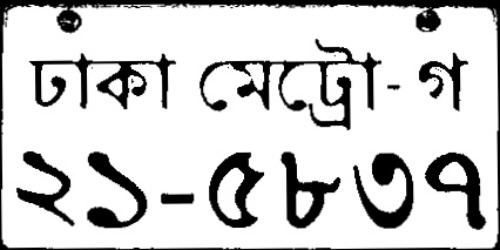
\includegraphics[width=.7\linewidth]{./img/sample/stage10.jpg}
    \caption{The extracted plate after rotation and scaling}
    \label{fig:FinalPlate}
\end{figure}



\end{document}
  \documentclass{standalone}
\usepackage{standalone}

\begin{document}

\subsection{Converting to Binary Image}
The image from previous stage is need to be converted in binary for convenience. Bangladeshi license plates have two types: white text on black plate for private cars and black text on white plate for public ones. To be accurate, we first converted the image into black and white using two filters: $THRESH_BINARY$ one time and $THRESH_BINARY_INV$ the other. Then compared the ratio of non-zero pixels of each image. The image which has lesser ratio, most probably is selected as the expected binary image. 

Figure \ref{fig:BlackAndWhite} shows the conversion to binary images using the above algorithm for different types of license plates.

\begin{figure}
\begin{subfigure}{.5\textwidth}
  \centering
  
\includegraphics[width=.8\linewidth]{./img/sample/bnw-1.jpg}
  \caption{A private license plate}
  \label{fig:PrivatePlate}
\end{subfigure}
\begin{subfigure}{.5\textwidth}
  \centering
  
\includegraphics[width=.8\linewidth]{./img/sample/bnw-2.jpg}
  \caption{Black and white image of \ref{fig:PrivatePlate}}
\end{subfigure}
\begin{subfigure}{.5\textwidth}
  \centering
  
\includegraphics[width=.8\linewidth]{./img/sample/bnw-3.jpg}
  \caption{A public license plate}
  \label{fig:PublicPlate}
\end{subfigure}
\begin{subfigure}{.5\textwidth}
  \centering
  
\includegraphics[width=.8\linewidth]{./img/sample/bnw-4.jpg}
  \caption{Black and white image of \ref{fig:PublicPlate}}
\end{subfigure}
\caption{Black and white conversion of two types of image}
\label{fig:BlackAndWhite}
\end{figure}


\end{document}
  \documentclass{standalone}
\usepackage{standalone}

\begin{document}
\subsection{Denoising}

\subsubsection{Border Removal}
Removing the borders of an image is tough job due to the diversity of plates and their origins. In our methods, we first removed the top, bottom, left and right border using OpenCV's $floodFill$ function. We checked all the pixels of first $20$ rows and applied flood-fill on any non-black pixels. Similarly we check bottom $5$ rows, from left first $12$ columns and from right the first $12$ columns.

\subsubsection{Contour cleaning}
Only removing border is not enough to completely clear the plate image. We used contour analysis to blackout the remaining dots in the image that could not possibly be a letter. To find contour, we used $cv2.RETR_EXTERNAL$ mode which only wraps the external area (Otherwise the holes inside numbers and letters would be detected, and it would pose a problem).

After some observation, we set the minimum character height to be between $35$ to $height-30$ pixels and width between $35$ to $width-30$. We checked for all contours if it a possible character. If not, we used OpenCV's $fillConvexPoly$ method on $minAreaRect$ of the contour. It nicely fill up the contour with black pixels and hide it without affecting rest of the plate image.


Figure \ref{fig:CleaningStage} shows the effects of this algorithm.
\begin{figure}
\begin{subfigure}{.5\textwidth}
  \centering
  
\includegraphics[width=.8\linewidth]{./img/sample/stage11.jpg}
  \caption{Noisy image}
\end{subfigure}
\begin{subfigure}{.5\textwidth}
  \centering
  
\includegraphics[width=.8\linewidth]{./img/sample/stage12.jpg}
  \caption{Removed borders}
\end{subfigure}
\begin{subfigure}{0.9\textwidth}
  \centering
  
\includegraphics[width=.8\linewidth]{./img/sample/stage13.jpg}
  \caption{Clean image}
\end{subfigure}
\caption{After applying Border removal and contour cleaning}
\label{fig:CleaningStage}
\end{figure}

\end{document}

\documentclass{standalone}
\usepackage{standalone}

\begin{document}
\section{Segmentation}
\subsection{Horizontal Segmentation}
\subsection{Vertical Segmentation}

\end{document}

\documentclass{standalone}
\usepackage{standalone}

\begin{document}

\section{Character Recognition}


\end{document}

\end{document}
\documentclass{standalone}
\usepackage{standalone}

\begin{document}
\chapter{Data Sets}
This section will introduce to our collected dataset in brief. 

\subsection{Variety of Images}
An image of a car can vary in many ways. Here are some of possible reason for variance:
\begin{itemize}
    \item Positions of plate varies in cars to cars.
    \item Colors of plates are different in many cars.
    \item Non-standard use of fonts.
    \item Materials of plates.
    \item Muds on license plate.
    \item Erased characters on plates.
    \item Due to the conditions of weather and time of the day, the light may prove a significant factor of variance. 
    \item The sun may create reflection on the license plates.
    \item Due to bumper-guards, the plate may be hidden in some cars.
    \item Image size may vary depending on the camera type.
    \item Resolution of the image taken may vary.
    \item Types and colors of plate puts an effect in plate image.
\end{itemize}

\subsection{Collected Dataset}
Due to the different conditions it is very difficult to collect a good enough data sets to properly capture all conditions. The conditions and variety of our dataset is represent in Table \ref{table:Variety}. Note that, same image fall into more than one category in the table below and the count was done in that way. 

\begin{table}    
    \caption{Data-set for experimentation}
    \label{table:Variety}
    \begin{tabular}{|l|r|}
    \hline
    {\bf Variety}  &  {\bf Number Of Images} \\ 
    \hline 
    In good condition &  42 \\ 
    Highly angled/skewed plate & 16 \\
    Bad Resolution & 19 \\ 
    Non-Standard Plates &  18\\    
    Private Vehicle & 8 \\
    Shadowed license plate & 11 \\    
    Light reflection & 9 \\
    Small plates & 6\\
    Muddy, erased or hidden letters & 18 \\
    Unrecognizable plates (for the bumper, mud, light etc.) & 14  \\
    \hline
    {\bf Total plates} & {\bf 138} \\
    \hline
    \end{tabular}
\end{table}

In our experimentation, we did not keep Unrecognizable plate images, and removed some bad quality images. Our final dataset was consists of $78$ images of different categories.

\subsection{Image samples}
Some sample images we used during our experimentation are shown in following figures (Figure \ref{fig:DataSamples1}).


\begin{figure}
\begin{subfigure}{0.5\textwidth}
    \centering
    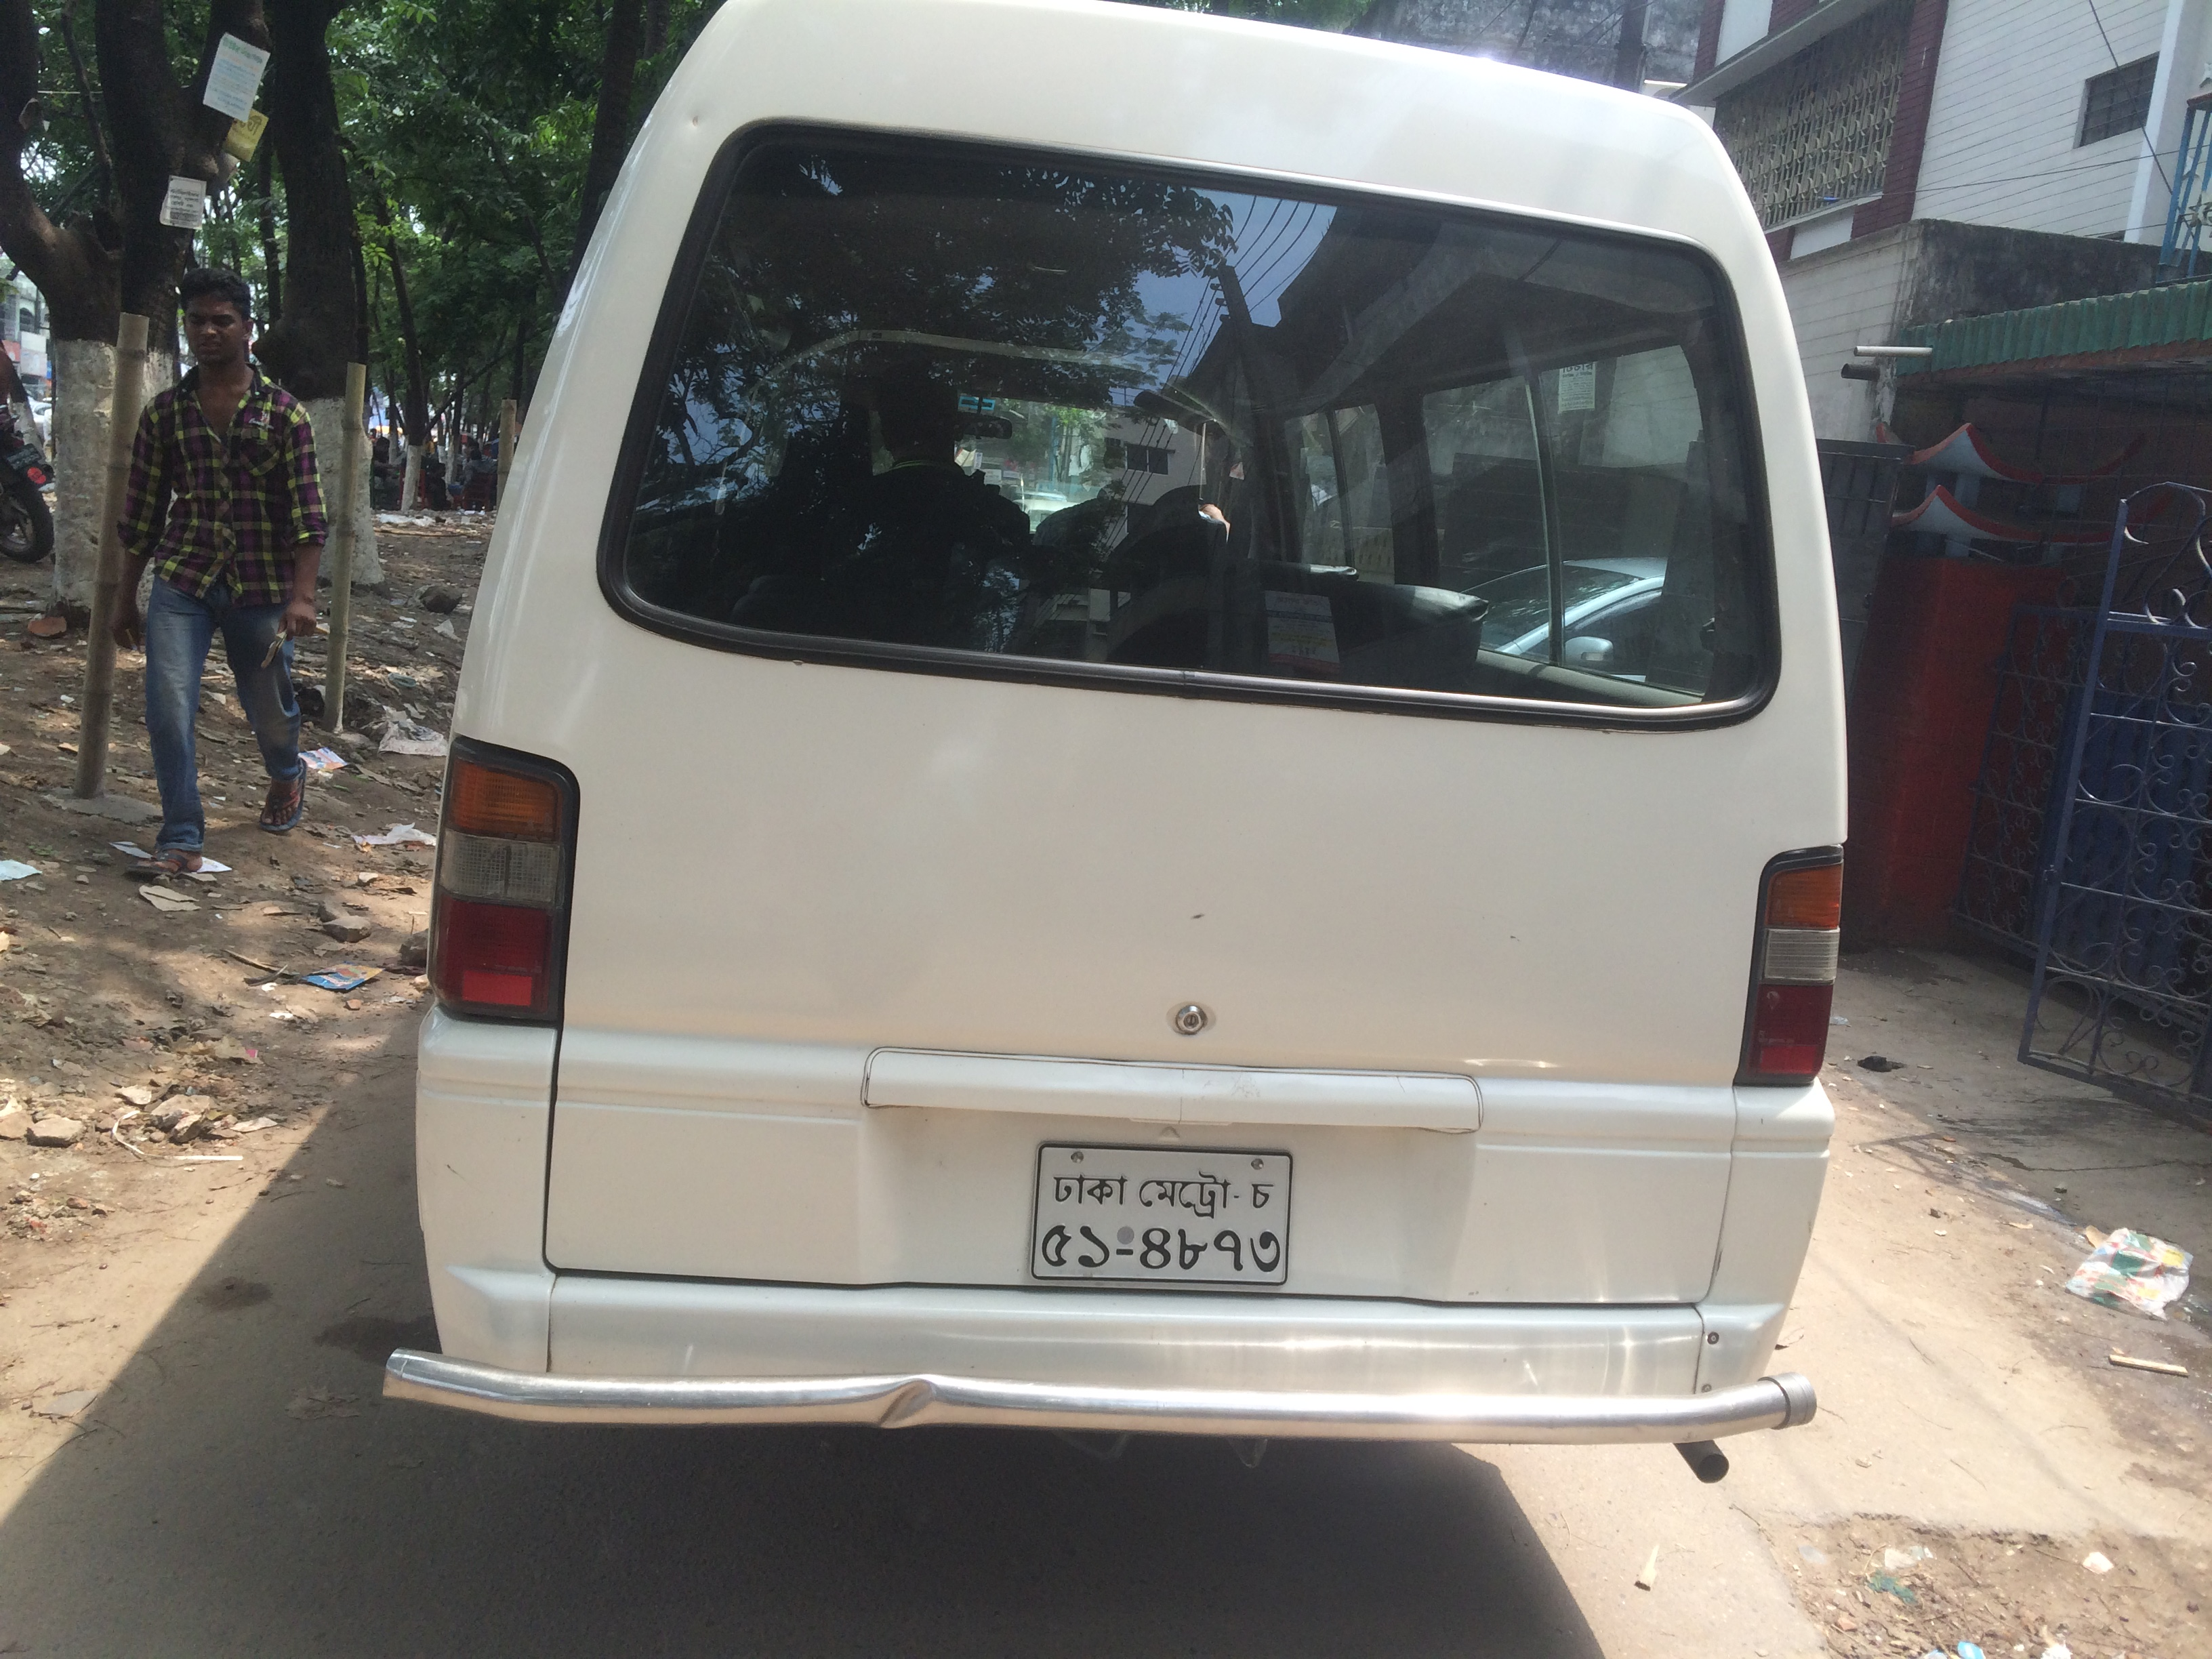
\includegraphics[width=0.8\linewidth]{./img/experiment/stage.0/angle}
    \caption{Thin letters}
\end{subfigure}
\begin{subfigure}{0.5\textwidth}
    \centering
    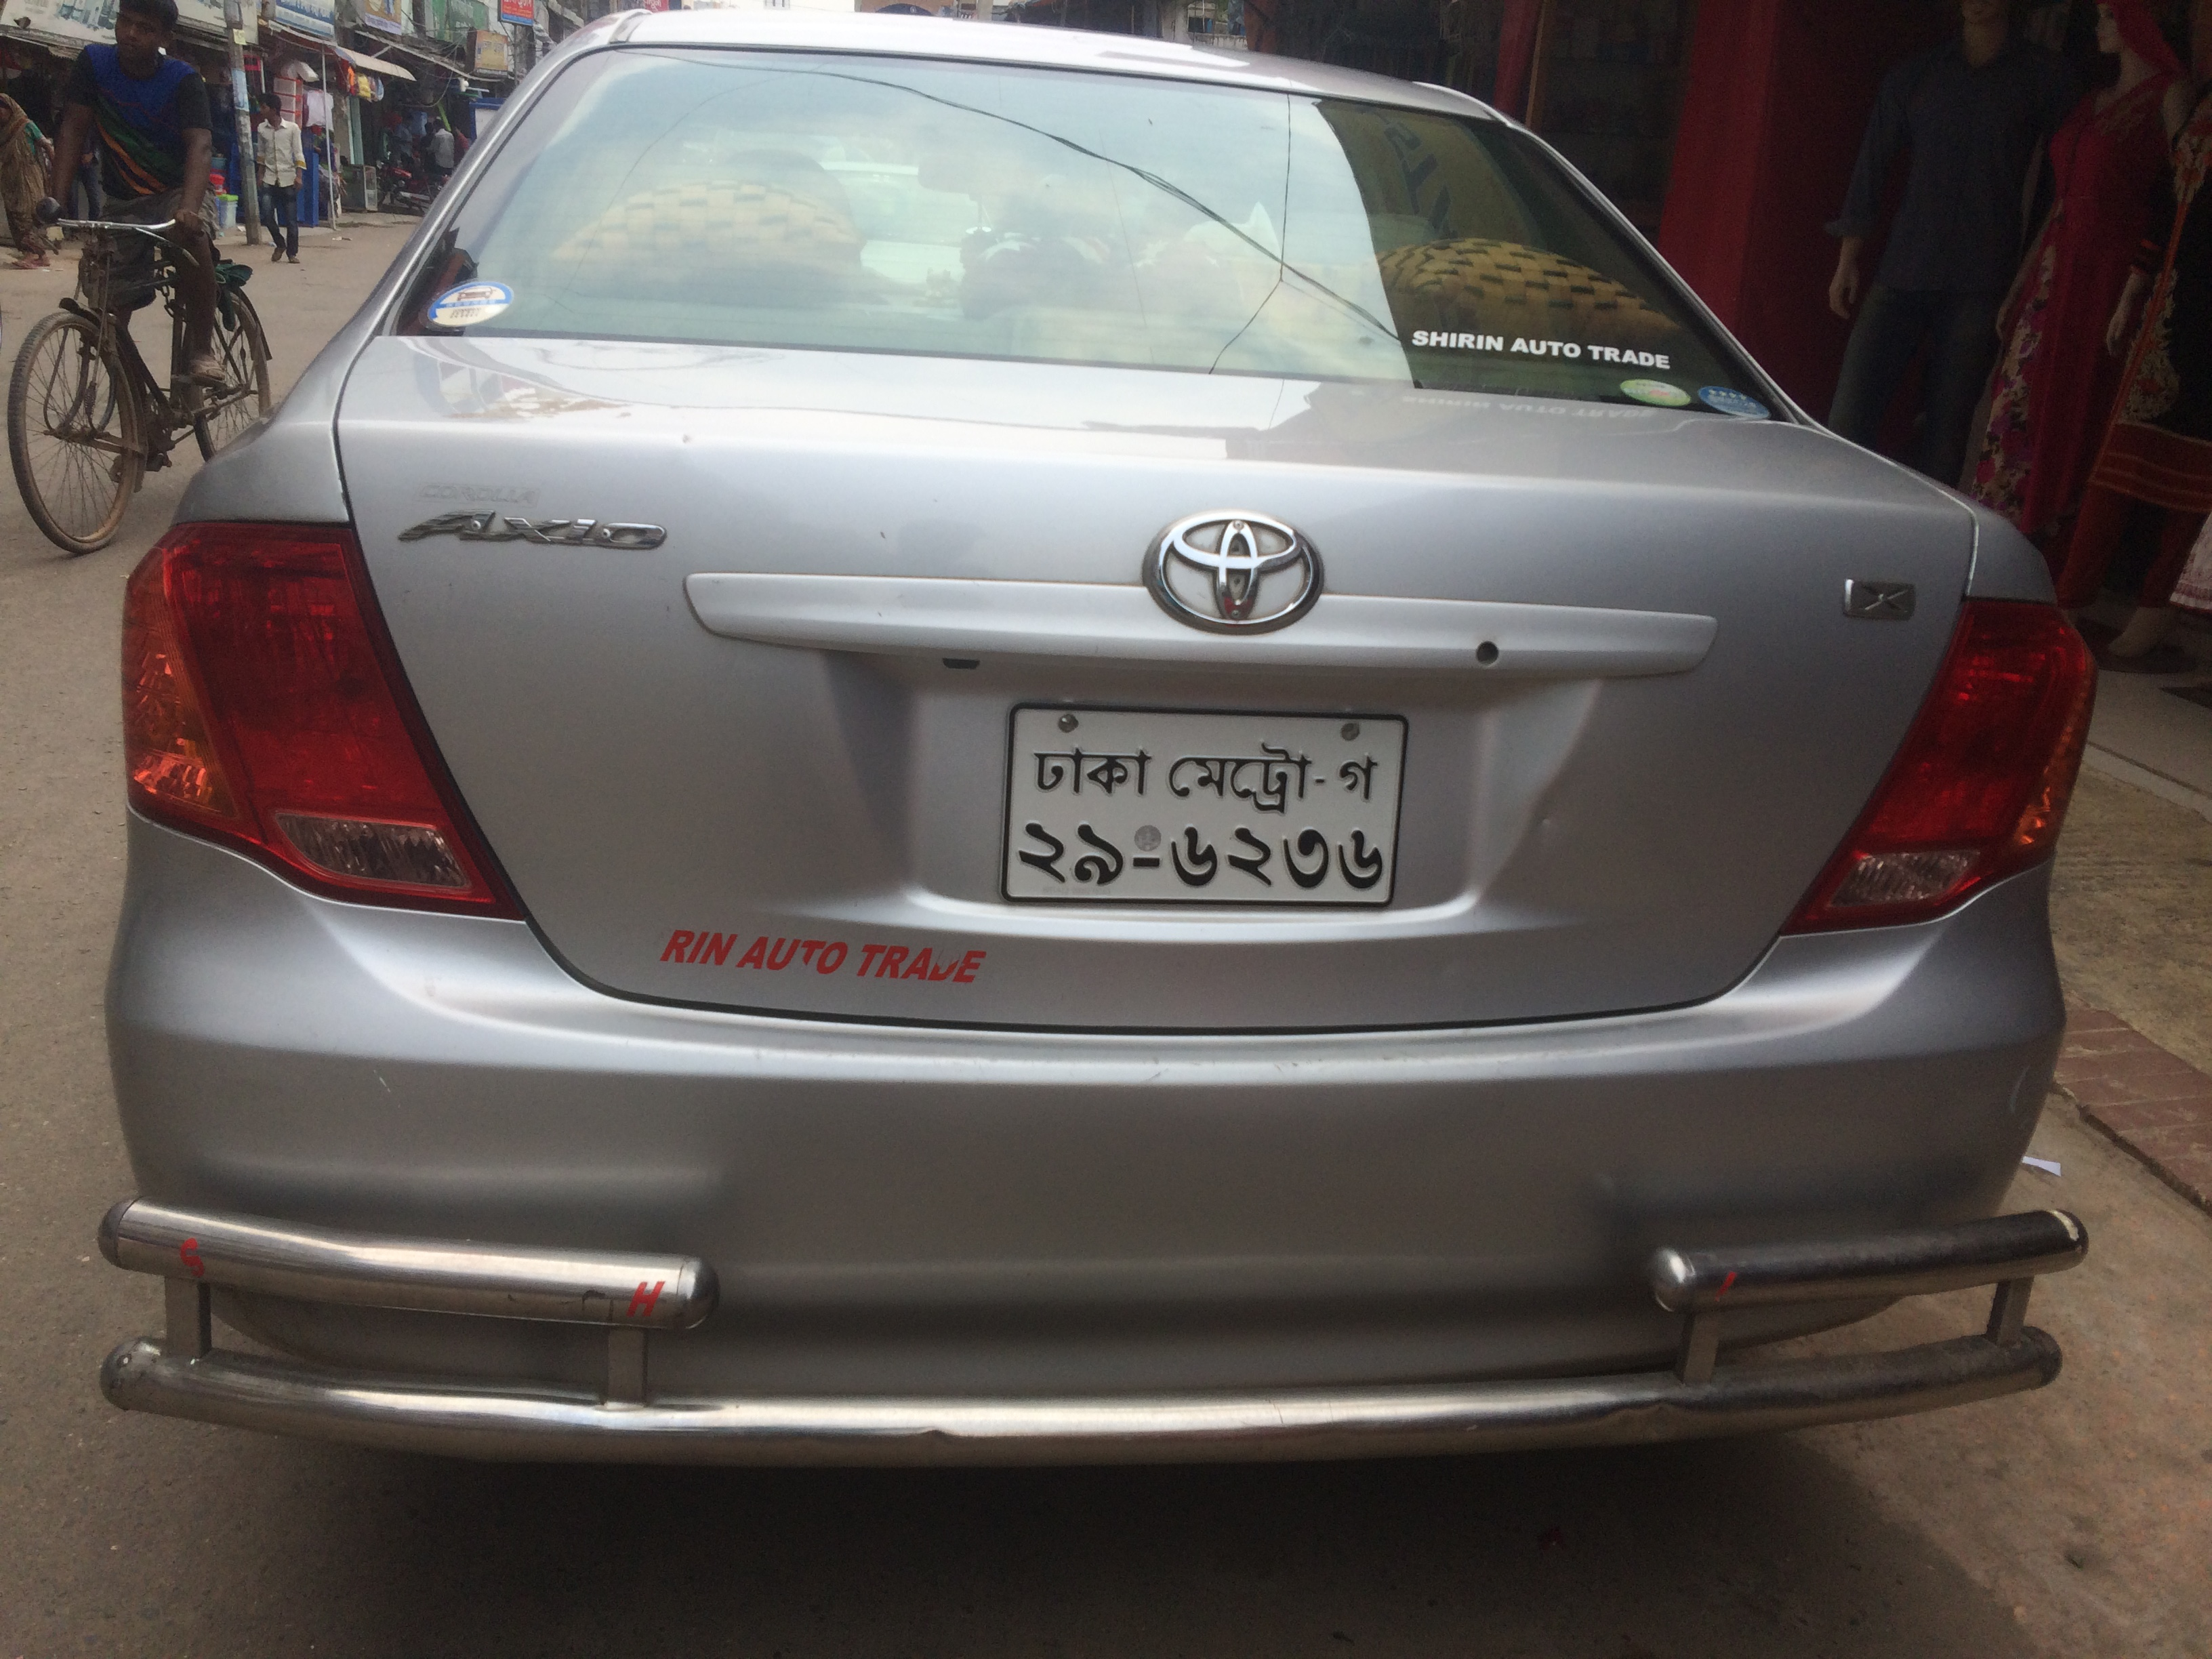
\includegraphics[width=0.8\linewidth]{./img/experiment/stage.0/angle2}
    \caption{Medium quality letters}
\end{subfigure}
\begin{subfigure}{1.0\textwidth}
    \centering
    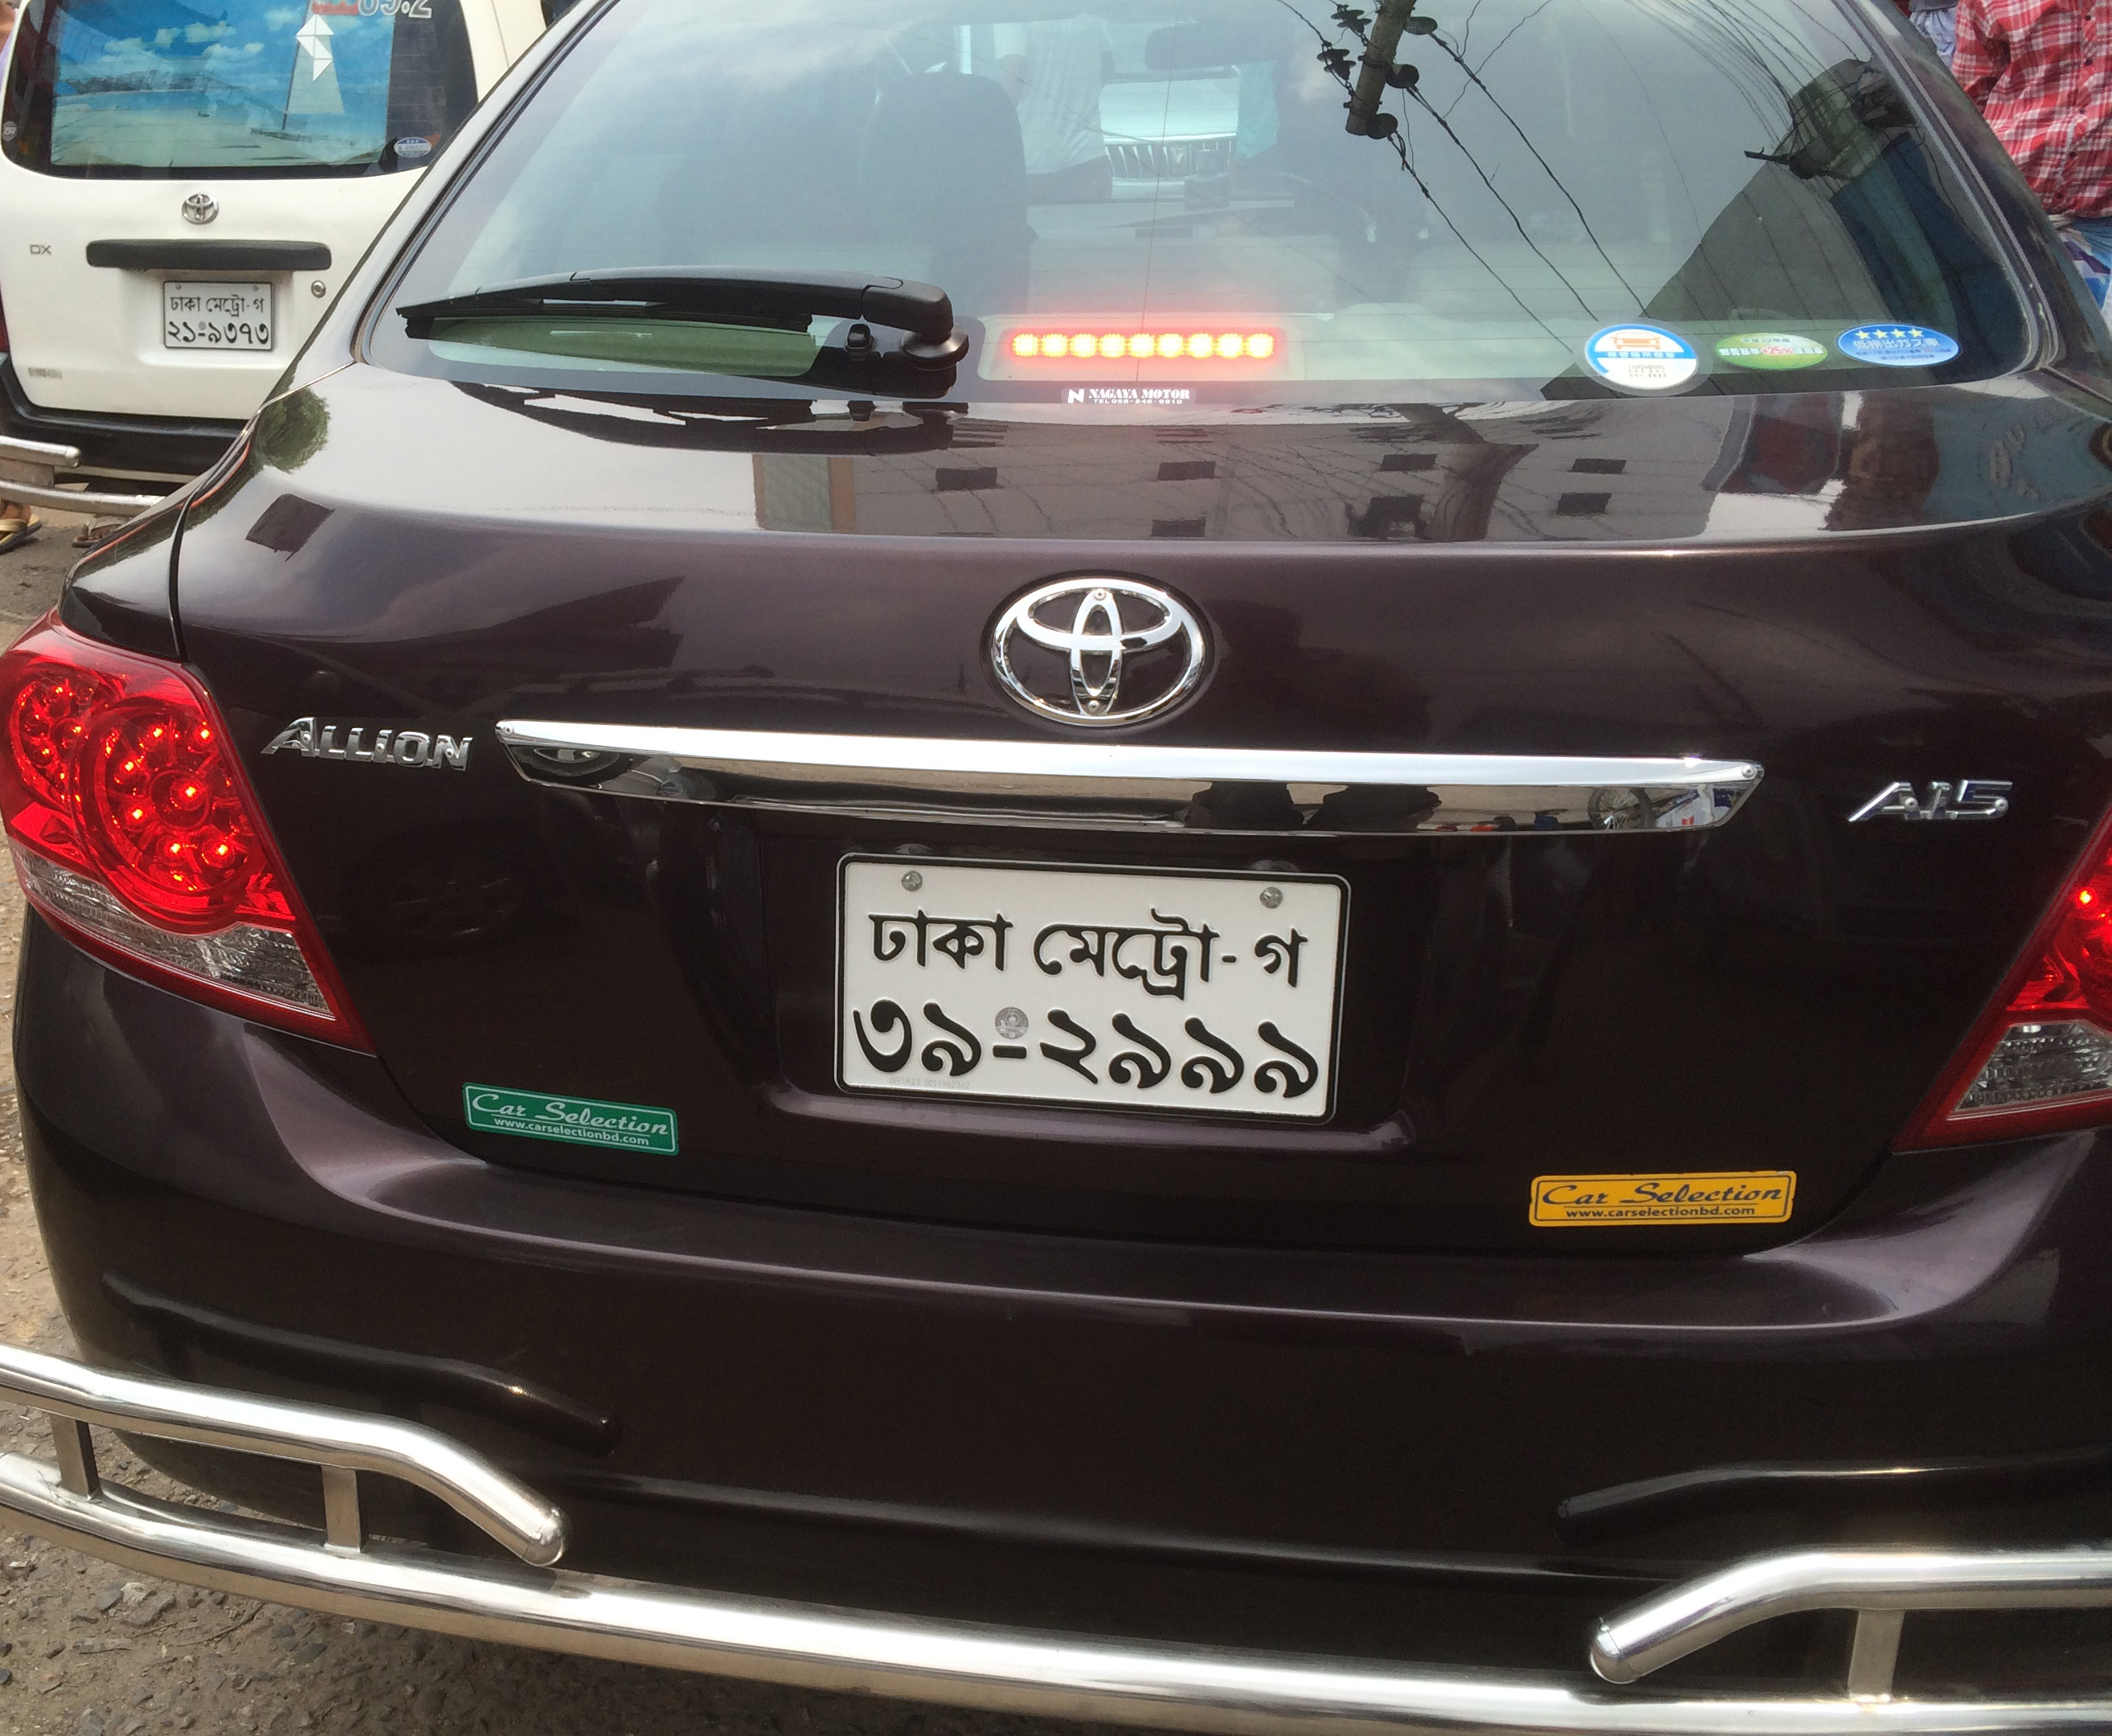
\includegraphics[width=0.8\linewidth]{./img/experiment/stage.0/angle3}
    \caption{High quality letters}
\end{subfigure}
\caption{Slightly angled license plates}
\label{fig:DataSamples1}
\end{figure}

\end{document}
\documentclass{standalone}
\usepackage{standalone}

\begin{document}
\chapter{Experiment and Results}
Our experiment process and the results will be shown in this chapter. We shall display our result for every significant stages in separate sections along with different types of samples.


\section{Preprocessing Stage}
This stage ends up generating a bunch of predicted license plate images. We shall show our output for some significant steps.
  
  \subsection{Edge Density Analysis}
This step analyzes edges using vertical Sobel operator from Gray-scale images. Figure \ref{fig:SobelResult1}, \ref{fig:SobelResult2}, and \ref{fig:SobelResult3} demonstrate the result we found after applying vertical Sobel filter on the original Gray-scale images.

\begin{figure}
\begin{subfigure}{0.5\textwidth}
    \centering
    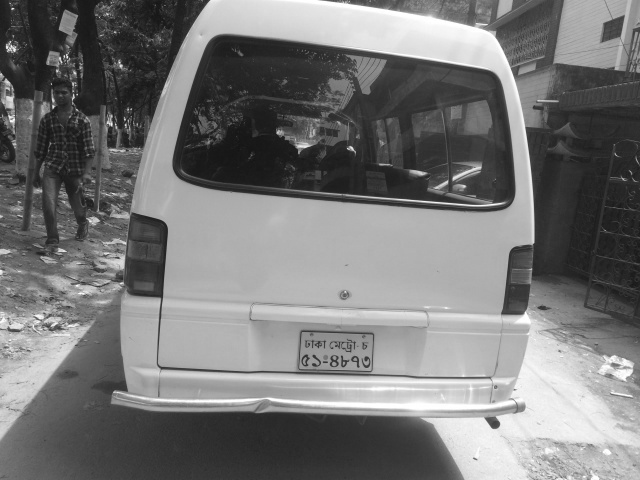
\includegraphics[width=0.9\linewidth]{./img/experiment/stage.2/angle}
    \caption{Original image}
\end{subfigure}
\begin{subfigure}{0.5\textwidth}
    \centering
    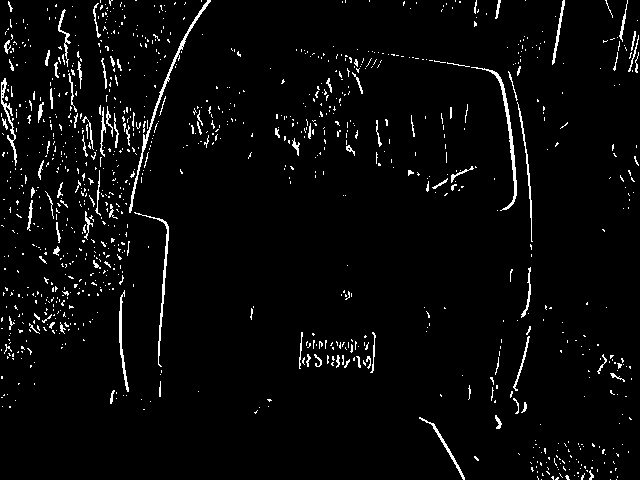
\includegraphics[width=0.9\linewidth]{./img/experiment/stage.3/angle}
    \caption{Edge image}
\end{subfigure}
\caption{Sobel image of a car with a slightly angled plate}
\label{fig:SobelResult1}
\end{figure}

\begin{figure}
\begin{subfigure}{0.5\textwidth}
    \centering
    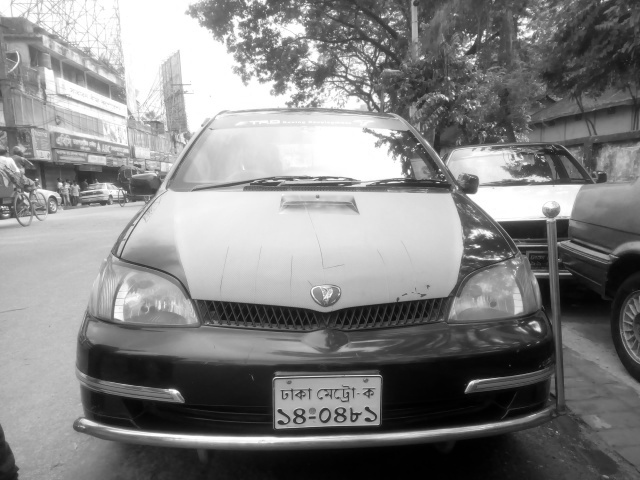
\includegraphics[width=0.9\linewidth]{./img/experiment/stage.2/good3}
    \caption{Original image}
\end{subfigure}
\begin{subfigure}{0.5\textwidth}
    \centering
    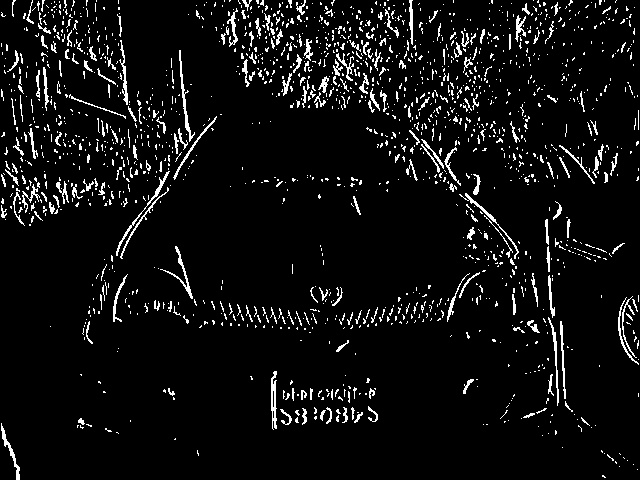
\includegraphics[width=0.9\linewidth]{./img/experiment/stage.3/good3}
    \caption{Edge image}
\end{subfigure}
\caption{Sobel image of a good plate image}
\label{fig:SobelResult2}
\end{figure}


\begin{figure}
\begin{subfigure}{0.5\textwidth}
    \centering
    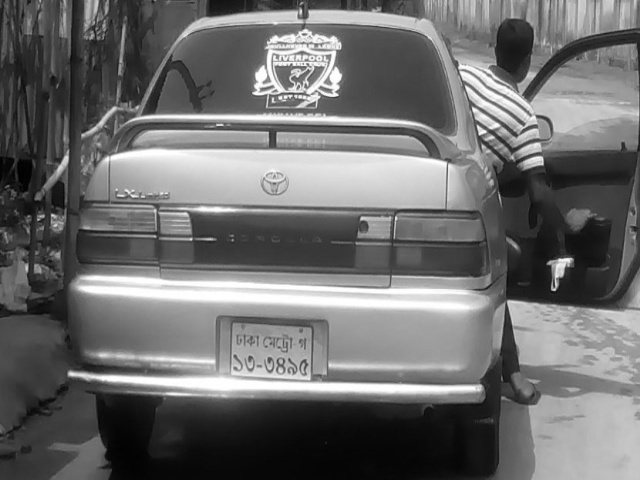
\includegraphics[width=0.9\linewidth]{./img/experiment/stage.2/light}
    \caption{Original image}
\end{subfigure}
\begin{subfigure}{0.5\textwidth}
    \centering
    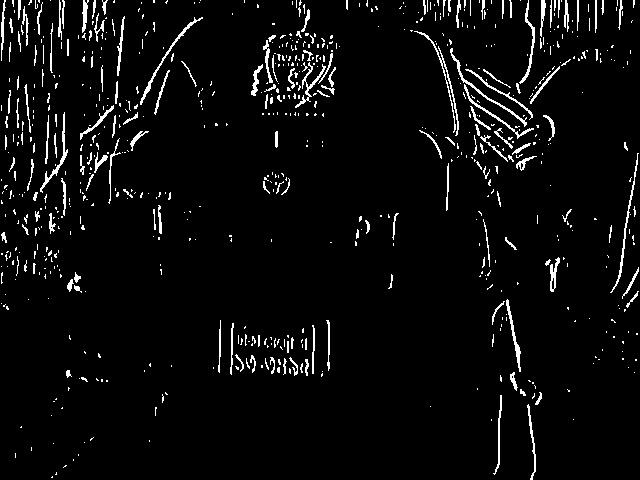
\includegraphics[width=0.9\linewidth]{./img/experiment/stage.3/light}
    \caption{Edge image}
\end{subfigure}
\caption{Sobel image of plate with light reflection}
\label{fig:SobelResult3}
\end{figure}

  \subsection{Gaussian Filter on Edge Image}
The Gaussian filter blurs the image. We observed that our filter blurs all of license plates on good samples, and only text portions on samples with larger plates. Figure \ref{fig:GaussianResult1}, \ref{fig:GaussianResult2} and \ref{fig:GaussianResult3} demonstrate result of this filter.

\begin{figure}
\begin{subfigure}{0.5\textwidth}
    \centering
    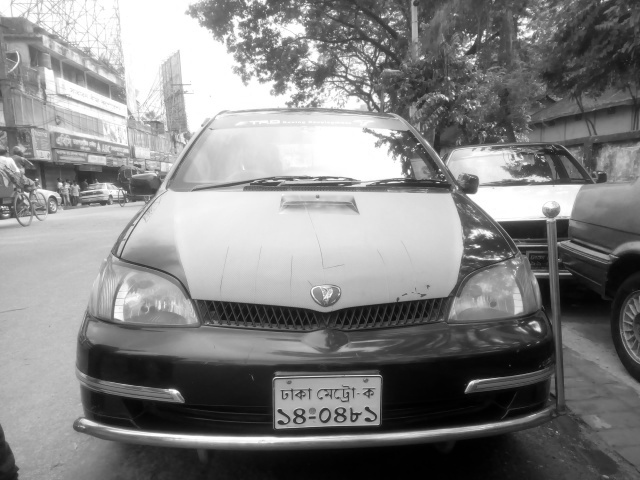
\includegraphics[width=0.9\linewidth]{./img/experiment/stage.2/good3}
    \caption{Original image}
\end{subfigure}
\begin{subfigure}{0.5\textwidth}
    \centering
    \includegraphics[width=0.9\linewidth]{./img/experiment/stage.4/good3}
    \caption{Blurry image}
\end{subfigure}
\caption{Gaussian filter on good plate}
\label{fig:GaussianResult1}
\end{figure}

\begin{figure}
\begin{subfigure}{0.5\textwidth}
    \centering
    \includegraphics[width=0.9\linewidth]{./img/experiment/stage.2/angle3}
    \caption{Original image}
\end{subfigure}
\begin{subfigure}{0.5\textwidth}
    \centering
    \includegraphics[width=0.9\linewidth]{./img/experiment/stage.4/angle3}
    \caption{Blurry image}
\end{subfigure}
\caption{Gaussian filter on big plate}
\label{fig:GaussianResult2}
\end{figure}

\begin{figure}
\begin{subfigure}{0.5\textwidth}
    \centering
    \includegraphics[width=0.9\linewidth]{./img/experiment/stage.2/small}
    \caption{Original image}
\end{subfigure}
\begin{subfigure}{0.5\textwidth}
    \centering
    \includegraphics[width=0.9\linewidth]{./img/experiment/stage.4/small}
    \caption{Blurry image}
\end{subfigure}
\caption{Gaussian filter on small plate}
\label{fig:GaussianResult3}
\end{figure}

  \subsection{Enhanced Image vs original image}
If images are skewed or angled, this step does not work so well. Also, for small images and other images which has low blur around plate regions enhanced margin is low. Figure \ref{fig:EnhanceResult1}, \ref{fig:EnhanceResult2}, \ref{fig:EnhanceResult3} and \ref{fig:EnhanceResult4} demonstrate result of this step.

\begin{figure}
\begin{subfigure}{0.5\textwidth}
    \centering
    \includegraphics[width=0.9\linewidth]{./img/experiment/stage.2/angle3}
    \caption{Original image}
\end{subfigure}
\begin{subfigure}{0.5\textwidth}
    \centering
    \includegraphics[width=0.9\linewidth]{./img/experiment/stage.5/angle3}
    \caption{Blurry image}
\end{subfigure}
\caption{Gaussian filter on good plate}
\label{fig:EnhanceResult1}
\end{figure}

\begin{figure}
\begin{subfigure}{0.5\textwidth}
    \centering
    \includegraphics[width=0.9\linewidth]{./img/experiment/stage.2/light}
    \caption{Original image}
\end{subfigure}
\begin{subfigure}{0.5\textwidth}
    \centering
    \includegraphics[width=0.9\linewidth]{./img/experiment/stage.5/light}
    \caption{Blurry image}
\end{subfigure}
\caption{Gaussian filter on plate with reflection}
\label{fig:EnhanceResult2}
\end{figure}

\begin{figure}
\begin{subfigure}{0.5\textwidth}
    \centering
    \includegraphics[width=0.9\linewidth]{./img/experiment/stage.2/small}
    \caption{Original image}
\end{subfigure}
\begin{subfigure}{0.5\textwidth}
    \centering
    \includegraphics[width=0.9\linewidth]{./img/experiment/stage.5/small}
    \caption{Blurry image}
\end{subfigure}
\caption{Gaussian filter on small plate}
\label{fig:EnhanceResult3}
\end{figure}


\begin{figure}
\begin{subfigure}{0.5\textwidth}
    \centering
    \includegraphics[width=0.9\linewidth]{./img/experiment/stage.2/angle}
    \caption{Original image}
\end{subfigure}
\begin{subfigure}{0.5\textwidth}
    \centering
    \includegraphics[width=0.9\linewidth]{./img/experiment/stage.5/angle}
    \caption{Blurry image}
\end{subfigure}
\caption{Gaussian filter on plate that is angled slightly}
\label{fig:EnhanceResult4}
\end{figure}

  \subsection{Matched filter on enhanced image}
Figure \ref{fig:MatchedResult1}, {fig:MatchedResult2}, {fig:MatchedResult3} show the result of this step.

\begin{figure}
\begin{subfigure}{0.5\textwidth}
    \centering
    \includegraphics[width=0.9\linewidth]{./img/experiment/stage.6/good}
    \caption{Final result}
\end{subfigure}
\begin{subfigure}{0.5\textwidth}
    \centering
    \includegraphics[width=0.9\linewidth]{./img/experiment/stage.6/3-good}
    \caption{A see-through view with original image}
\end{subfigure}
\caption{After applying matched filter on a good image}
\label{fig:MatchedResult1}
\end{figure}

\begin{figure}
\begin{subfigure}{0.5\textwidth}
    \centering
    \includegraphics[width=0.9\linewidth]{./img/experiment/stage.2/good3}
    \caption{Original image}
\end{subfigure}
\begin{subfigure}{0.5\textwidth}
    \centering
    \includegraphics[width=0.9\linewidth]{./img/experiment/stage.3/good3}
    \caption{Edge image}
\end{subfigure}
\caption{Sobel image of a good plate image}
\label{fig:MatchedResult2}
\end{figure}


\begin{figure}
\begin{subfigure}{0.5\textwidth}
    \centering
    \includegraphics[width=0.9\linewidth]{./img/experiment/stage.2/light}
    \caption{Original image}
\end{subfigure}
\begin{subfigure}{0.5\textwidth}
    \centering
    \includegraphics[width=0.9\linewidth]{./img/experiment/stage.3/light}
    \caption{Edge image}
\end{subfigure}
\caption{Sobel image of plate with light reflection}
\label{fig:MatchedResult3}
\end{figure}

  \subsection{Estimated plate regions}
Plate estimation is depended on the image found after applying matched filter. Bad plate images does not get enhanced well. Consequently it fails to have a good match on license plate regions and fails to locate exact positions of the plates. Good and bad results of this step is shown in Figure \ref{fig:Estimate1}, and \ref{fig:Estimate2}.

\begin{figure}
\begin{subfigure}{0.5\textwidth}
    \centering
    \includegraphics[width=0.9\linewidth]{./img/experiment/stage.2/good}
    \caption{Original image}
\end{subfigure}
\begin{subfigure}{0.5\textwidth}
    \centering
    \includegraphics[width=0.9\linewidth]{./img/experiment/stage.8/00-good}
    \caption{The only estimated plate region}
\end{subfigure}
\caption{A good example of plate estimation}
\label{fig:Estimate1}
\end{figure}


\begin{figure}
\begin{subfigure}{0.5\textwidth}
    \centering
    \includegraphics[width=0.9\linewidth]{./img/experiment/stage.2/private}
    \caption{Original image}
\end{subfigure}
\begin{subfigure}{0.24\textwidth}
    \centering
    \includegraphics[width=0.9\linewidth]{./img/experiment/stage.8/00-private}
    \\ \vspace{0.3cm}
    \includegraphics[width=0.9\linewidth]{./img/experiment/stage.8/02-private}
\end{subfigure}
\begin{subfigure}{0.24\textwidth}
    \centering
    \includegraphics[width=0.9\linewidth]{./img/experiment/stage.8/01-private}
    \\ \vspace{0.3cm}
    \includegraphics[width=0.9\linewidth]{./img/experiment/stage.8/03-private}
\end{subfigure}
\caption{Plate with lots of estimation}
\label{fig:Estimate2}
\end{figure}


\begin{figure}
\begin{subfigure}{0.5\textwidth}
    \centering
    \includegraphics[width=0.9\linewidth]{./img/experiment/stage.2/small}
    \caption{Original image}
\end{subfigure}
\begin{subfigure}{0.24\textwidth}
    \centering
    \includegraphics[width=0.9\linewidth]{./img/experiment/stage.8/00-small}
    \\ \vspace{0.3cm}
    \includegraphics[width=0.9\linewidth]{./img/experiment/stage.8/02-small}
\end{subfigure}
\begin{subfigure}{0.24\textwidth}
    \centering
    \includegraphics[width=0.9\linewidth]{./img/experiment/stage.8/01-small}
\end{subfigure}
\caption{Bad estimations}
\label{fig:Estimate2}
\end{figure}




\section{Plate Detection}
It takes every predicted plates and keeps only the text part of the plates. It also removes plates that can not be a possible plate.

  \subsection{Canny Edge Algorithm}
This algorithm is almost perfect for in detecting plate boundary. But if the plate is skewed or angled more tan 10 degrees it fails to draw a perfect boundary. In cases where the boundary is not inside the located region it also fails. Another backdrop is it draws double boundary for a plate for most of the cases. 

In Figure \ref{fig:CannyResult1}, \ref{fig:CannyResult2}, \ref{fig:CannyResult3}, and \ref{fig:CannyResult4} the results of the algorithm is shown.



\begin{figure}
\begin{subfigure}{0.33\textwidth}
    \centering
    \includegraphics[width=0.9\linewidth]{./img/experiment/stage.9/00-good}
    \caption{Original}
\end{subfigure}
\begin{subfigure}{0.33\textwidth}
    \centering
    \includegraphics[width=0.9\linewidth]{./img/experiment/stage.10/00-good}
    \caption{Threshold applied}
\end{subfigure}
\begin{subfigure}{0.33\textwidth}
    \centering
    \includegraphics[width=0.9\linewidth]{./img/experiment/stage.11/00-good}
    \caption{Canny edges}
\end{subfigure}
\caption{Canny edges of a good plate}
\label{fig:CannyResult1}
\end{figure}


\begin{figure}
\begin{subfigure}{0.33\textwidth}
    \centering
    \includegraphics[width=0.9\linewidth]{./img/experiment/stage.9/00-angle2}
    \caption{Original}
\end{subfigure}
\begin{subfigure}{0.33\textwidth}
    \centering
    \includegraphics[width=0.9\linewidth]{./img/experiment/stage.10/00-angle2}
    \caption{Threshold applied}
\end{subfigure}
\begin{subfigure}{0.33\textwidth}
    \centering
    \includegraphics[width=0.9\linewidth]{./img/experiment/stage.11/00-angle2}
    \caption{Canny edges}
\end{subfigure}
\caption{Canny edges of an angled plate}
\label{fig:CannyResult2}
\end{figure}

\begin{figure}
\begin{subfigure}{0.33\textwidth}
    \centering
    \includegraphics[width=0.9\linewidth]{./img/experiment/stage.9/02-private}
    \caption{Original}
\end{subfigure}
\begin{subfigure}{0.33\textwidth}
    \centering
    \includegraphics[width=0.9\linewidth]{./img/experiment/stage.10/02-private}
    \caption{Threshold applied}
\end{subfigure}
\begin{subfigure}{0.33\textwidth}
    \centering
    \includegraphics[width=0.9\linewidth]{./img/experiment/stage.11/02-private}
    \caption{Canny edges}
\end{subfigure}
\caption{Canny edges of a private plate}
\label{fig:CannyResult3}
\end{figure}


\begin{figure}
\begin{subfigure}{0.33\textwidth}
    \centering
    \includegraphics[width=0.9\linewidth]{./img/experiment/stage.9/02-small}
    \caption{Original}
\end{subfigure}
\begin{subfigure}{0.33\textwidth}
    \centering
    \includegraphics[width=0.9\linewidth]{./img/experiment/stage.10/02-small}
    \caption{Threshold applied}
\end{subfigure}
\begin{subfigure}{0.33\textwidth}
    \centering
    \includegraphics[width=0.9\linewidth]{./img/experiment/stage.11/02-small}
    \caption{Canny edges}
\end{subfigure}
\caption{Canny edges of a bad estimation}
\label{fig:CannyResult4}
\end{figure}


  \subsection{Contour Analysis}
The detection of contours vastly depended on the quality of edges detected by Canny edge detection algorithm. The contours can detect rotation, but we did not include the skew calculation. Rotation value fails in cases when the border of plate is not detected well or is out of the boundary of located plate region.

Figure \ref{fig:ContourResult1}, and \ref{fig:ContourResult2} shows two detected contour regions in each image. Contours are marked with a line of 2 pixels of black border upon 3 pixels of white border line.

\begin{figure}
\centering
\includegraphics[width=0.8\textwidth]{./img/experiment/stage.12/00-good}   
\caption{Two detected contours of a good sample}
\label{fig:ContourResult1}
\end{figure}

\begin{figure}
\centering
\includegraphics[width=0.8\textwidth]{./img/experiment/stage.12/00-private2}
\caption{Detected contours of a private plate}
\label{fig:ContourResult2}
\end{figure}


  \subsection{Extracted plates}
The extracted plate is also rotated according on contour data. If the contour fails to be detected properly, this also fails. Figure \ref{fig:ExtractedResult1}, \ref{fig:ExtractedResult2}, \ref{fig:ExtractedResult3}, and \ref{fig:ExtractedResult4} have some experimental results of the extracted plates.

\begin{figure}
\begin{subfigure}{0.5\textwidth}
    \centering
    \includegraphics[width=0.9\linewidth]{./img/experiment/stage.10/00-good}
    \caption{Original Plate}
\end{subfigure}
\begin{subfigure}{0.5\textwidth}
    \centering
    \includegraphics[width=0.9\linewidth]{./img/experiment/stage.13/00-00-good}
    \caption{Sole extracted image}
\end{subfigure}
\caption{Extracted parts of a good estimation}
\label{fig:ExtractedResult1}
\end{figure}

\begin{figure}
\begin{subfigure}{\textwidth}
    \centering
    \includegraphics[width=0.5\linewidth]{./img/experiment/stage.10/00-good3}
    \caption{Original Plate}
\end{subfigure}
\begin{subfigure}{0.5\textwidth}
    \centering
    \includegraphics[width=0.9\linewidth]{./img/experiment/stage.13/00-00-good3}
    \caption{First extracted image}    
\end{subfigure}
\begin{subfigure}{0.5\textwidth}
    \centering
    \includegraphics[width=0.9\linewidth]{./img/experiment/stage.13/01-00-good3}
    \caption{Second extracted image}
\end{subfigure}
\caption{Extracted parts of another good estimation}
\label{fig:ExtractedResult2}
\end{figure}


\begin{figure}
\begin{subfigure}{\textwidth}
    \centering
    \includegraphics[width=0.5\linewidth]{./img/experiment/stage.10/00-angle}
    \caption{Original Plate}
\end{subfigure}
\begin{subfigure}{0.5\textwidth}
    \centering
    \includegraphics[width=0.9\linewidth]{./img/experiment/stage.13/00-00-angle}
    \caption{First extracted image}
\end{subfigure}
\begin{subfigure}{0.5\textwidth}
    \centering
    \includegraphics[width=0.9\linewidth]{./img/experiment/stage.13/01-00-angle}
    \caption{Second extracted image}
\end{subfigure}
\caption{Extracted parts of angled plate}
\label{fig:ExtractedResult3}
\end{figure}


\begin{figure}
\begin{subfigure}{\textwidth}
    \centering
    \includegraphics[width=0.5\linewidth]{./img/experiment/stage.10/02-private}
    \caption{Original Plate}
\end{subfigure}
\begin{subfigure}{0.5\textwidth}
    \centering
    \includegraphics[width=0.9\linewidth]{./img/experiment/stage.13/00-02-private}
    \caption{First extracted image}
\end{subfigure}
\begin{subfigure}{0.5\textwidth}
    \centering
    \includegraphics[width=0.9\linewidth]{./img/experiment/stage.13/01-02-private}
    \caption{Second extracted image}
\end{subfigure}
\caption{Extracted parts of a private plate}
\label{fig:ExtractedResult4}
\end{figure}




  \subsection{Clean Plates}
After extracting plates the plates are converted into binary. This process has no failures. However the cleaning part has some critical cases. When the text is too close border, a portion of it gets erased. Also, sometimes if noise density and size large it is assumed to be a character and does not get erased. All such cases are shown in Figure \ref{fig:Cleaning1}, \ref{fig:Cleaning2}, and \ref{fig:Cleaning3}.


\begin{figure}
\begin{subfigure}{0.33\textwidth}
    \centering
    \includegraphics[width=0.9\linewidth]{./img/experiment/stage.14/01-00-good}
    \caption{Binary image}
\end{subfigure}
\begin{subfigure}{0.33\textwidth}
    \centering
    \includegraphics[width=0.9\linewidth]{./img/experiment/stage.15/01-00-good}
    \caption{Removed Borders}
\end{subfigure}
\begin{subfigure}{0.33\textwidth}
    \centering
    \includegraphics[width=0.9\linewidth]{./img/experiment/stage.16/01-00-good}
    \caption{Final image}
\end{subfigure}
\caption{Result of good cleaning}
\label{fig:Cleaning1}
\end{figure}

\begin{figure}
\begin{subfigure}{0.33\textwidth}
    \centering
    \includegraphics[width=0.9\linewidth]{./img/experiment/stage.14/01-00-private2}
    \caption{Binary image}
\end{subfigure}
\begin{subfigure}{0.33\textwidth}
    \centering
    \includegraphics[width=0.9\linewidth]{./img/experiment/stage.15/01-00-private2}
    \caption{Removed Borders}
\end{subfigure}
\begin{subfigure}{0.33\textwidth}
    \centering
    \includegraphics[width=0.9\linewidth]{./img/experiment/stage.16/01-00-private2}
    \caption{Final image}
\end{subfigure}
\caption{Result of bad cleaning}
\label{fig:Cleaning2}
\end{figure}


\begin{figure}
\begin{subfigure}{0.33\textwidth}
    \centering
    \includegraphics[width=0.9\linewidth]{./img/experiment/stage.14/00-00-good3}
    \caption{Binary image}
\end{subfigure}
\begin{subfigure}{0.33\textwidth}
    \centering
    \includegraphics[width=0.9\linewidth]{./img/experiment/stage.15/00-00-good3}
    \caption{Removed Borders}
\end{subfigure}
\begin{subfigure}{0.33\textwidth}
    \centering
    \includegraphics[width=0.9\linewidth]{./img/experiment/stage.16/00-00-good3}
    \caption{Final image}
\end{subfigure}
\caption{Cleaning an skewed plate}
\label{fig:Cleaning3}
\end{figure}


  

\section{Segmentation}  
Horizontal and vertical project are not perfect for skewed and angled plates. It also fails in case there are induced noise on license plate. Also if two characters overlaps each other in vertical direction (which is very common in bangla text) it also fails. Figure \ref{fig:SegmentResult1} shows an example of successful segmentation. When two characters overlaps the segmentation fails. An example is shown in Figure \ref{fig:OverlappingChar}. Also, non-standard plate like Figure \ref{fig:NonStandardPlates}.


\begin{figure}
\begin{subfigure}{\textwidth}
    \centering
    \includegraphics[width=0.5\linewidth]{./img/experiment/stage.16/01-00-good}
    \caption{Original Plate}
\end{subfigure}
\begin{subfigure}{0.15\textwidth}
    \centering
    \includegraphics[width=0.9\linewidth]{./img/experiment/stage.17/00-01-00-good}
\end{subfigure}
\begin{subfigure}{0.15\textwidth}
    \centering
    \includegraphics[width=0.9\linewidth]{./img/experiment/stage.17/01-01-00-good}
\end{subfigure}
\begin{subfigure}{0.09\textwidth}
    \centering
    \includegraphics[width=0.9\linewidth]{./img/experiment/stage.17/02-01-00-good}
\end{subfigure}
\begin{subfigure}{0.09\textwidth}
    \centering
    \includegraphics[width=0.9\linewidth]{./img/experiment/stage.17/03-01-00-good}
\end{subfigure}
\begin{subfigure}{0.09\textwidth}
    \centering
    \includegraphics[width=0.9\linewidth]{./img/experiment/stage.17/04-01-00-good}
\end{subfigure}
\begin{subfigure}{0.09\textwidth}
    \centering
    \includegraphics[width=0.9\linewidth]{./img/experiment/stage.17/05-01-00-good}
\end{subfigure}
\begin{subfigure}{0.09\textwidth}
    \centering
    \includegraphics[width=0.9\linewidth]{./img/experiment/stage.17/06-01-00-good}
\end{subfigure}
\begin{subfigure}{0.09\textwidth}
    \centering
    \includegraphics[width=0.9\linewidth]{./img/experiment/stage.17/07-01-00-good}
\end{subfigure}
\begin{subfigure}{0.09\textwidth}
    \centering
    \includegraphics[width=0.9\linewidth]{./img/experiment/stage.17/08-01-00-good}
\end{subfigure}
\caption{Segmented characters from a plate}
\label{fig:SegmentResult1}
\end{figure}


\begin{figure}
\begin{subfigure}{0.33\textwidth}
    \centering
    \includegraphics[width=0.9\linewidth]{./img/experiment/stage.17/06-00-00-badfont}
    \caption{Bad font}
\end{subfigure}
\begin{subfigure}{0.33\textwidth}
    \centering
    \includegraphics[width=0.9\linewidth]{./img/experiment/stage.17/07-01-00-private2}
    \caption{Skewed}
\end{subfigure}
\begin{subfigure}{0.33\textwidth}
    \centering
    \includegraphics[width=0.9\linewidth]{./img/experiment/stage.17/06-01-02-private}
    \caption{Non-standard font}
\end{subfigure}
\caption{Segmentation failed due to overlapping characters}
\label{fig:OverlappingChar}
\end{figure}


\begin{figure}
\centering
\includegraphics[width=0.5\linewidth]{./img/experiment/stage.16/01-00-nostd}    
\caption{Segmentation fails for non-standard plates}
\label{fig:NonStandardPlates}
\end{figure}




\section{Character Recognition}
The character recognition is done by neural network which is highly depended on training dataset. Unfortunately, we did not have enough dataset to train our neural network well to be able to produce any significant results. Our future goal includes this part of collecting dataset, and training and testing the neural network we implemented.


\section{Efficiency Measurements}


\end{document}

%\documentclass{standalone}
\usepackage{standalone}

\begin{document}
	\chapter{Data Sets}
	\section{Data Sources}
	There we used mainly two data sets for reference and three data set for read. Among them, one synthetic reference data set and one read data set is generated by us randomly. Our generated data set for read contains fifty read sequences having length ten thousands each. Our reference is treated as \emph{Synthetic Reference} and reads are treated as \emph{Synthetic Reads} in the context.
	
	As a real data, we have taken \emph{GenBank: U00096.1} version of \emph{Escherichia coli K-12 MG1655 complete genome}\cite{ecoli_ref} which is freely available online.
	We have two read data sets for this reference genome. One is simulated by Ruhul Amin Shajib while developing NanoBLASTer \cite{nanoBLAST}. We called it \emph{20K Simulated Reads} or simply \emph{20K Reads} during the whole work and writings. The other data is treated as 25K reads which is collected from a source of data used in Minimap\cite{minimap}. The table \ref{tab:dataStat} shows a general statistics about the data sets.
	\begin{table}[ht]
		\centering
		\caption{Summary of Data Sets Used in The Experiments.}
		\label{tab:dataStat}
		\begin{tabular}{|c|>{\centering\arraybackslash}m{1.8cm}|m{0.9cm}|>{\centering\arraybackslash}m{1.4cm}|>{\centering\arraybackslash}m{2cm}|>{\centering\arraybackslash}m{1.5cm}|>{\centering\arraybackslash}m{1.5cm}|>{\centering\arraybackslash}m{1.7cm}|}
			\hline 
			\textbf{No} & \textbf{Name of Data Set} & \textbf{\# of Reads} & \textbf{\# of Usable Reads} & \textbf{Total Length of Reads} & \textbf{Average Length of Reads} & \textbf{Reference Name} & \textbf{Length of Reference} \\ \hline \hline
			1           & 20K Simulated Reads       & 20000                & 17043                       & 118335765                      & 6943.36                          & \textit{E. Coli}        & 4639211                      \\ \hline
			2           & 25K Reads                 & 25970                & 25970                       & 216906558                      & 8352.2                           & \textit{E. Coli}        & 4639211                      \\ \hline
			3           & Synthetic Reads           & 50                   & 50                          & 500000                         & 10000                            & Synthetic               & 493290                       \\ \hline
		\end{tabular}
	\end{table}
	\section{Error Rate in Data}
	\emph{20K Simulated Reads} data has some \emph{unaligned} reads which we totally ignored in experiment. This data set has 15\% to 45\% error in data. \emph{20K Reads} data has up to 15\% error.
	On the other hand, our \emph{Synthetic Reads} data has no error as we randomly picked a chunk of 10K base at a time. However, we have added a limited number of random errors which have described in the corresponding context.
\end{document}

%\documentclass{standalone}
\usepackage{standalone}

\begin{document}
\section{Comparison With Other Tools}
With error free data, NanoMapper works best. It could map exact positions and map only one position where other tools give some worng positions along with the right position. However, when error chunk added in the data, NanoMapper performs well. As mapping to wrong position could be misleading, a penalty should be added for this. It is not possible to check every base is mapped to the right position or not for certain reasons. In fact, tools map overlapped ranges. Considering all of these restrictions, the following equations are used to evaluate the accuracy.
$$\textbf{Right \%} = \frac{\textbf{\# of Base Mapped to Right Range}}{\textbf{Total \# of Mapped Base}}$$
Similarly,
$$\textbf{Wrong \%} = \frac{\textbf{\# of Base Mapped to Out of Right Range}}{\textbf{Total \# of Mapped Base}}$$

With 5\% error chunk added in the synthetic data, the result is like table \ref{tab:error5}.
\begin{table}[]
	\centering
	\caption{Mapping Comparison While 5\% Error Added in Read Data}
	\label{tab:error5}
	\begin{tabular}{|c|c|c|}
		\hline
		\begin{tabular}[c]{@{}c@{}}Name of the\\ Tool\end{tabular} & \begin{tabular}[c]{@{}c@{}}Right Position\\ (\%)\end{tabular} & \begin{tabular}[c]{@{}c@{}}Wrong Position\\ (\%)\end{tabular} \\ \hline
		BWA-MEM & 88.4 & 11.6 \\ \hline
		NanoBLAST & 86.55 & 13.45 \\ \hline
		NanoMapper & 97.42 & 2.58 \\ \hline
	\end{tabular}
\end{table}

\begin{figure}
	\centering
	
	
	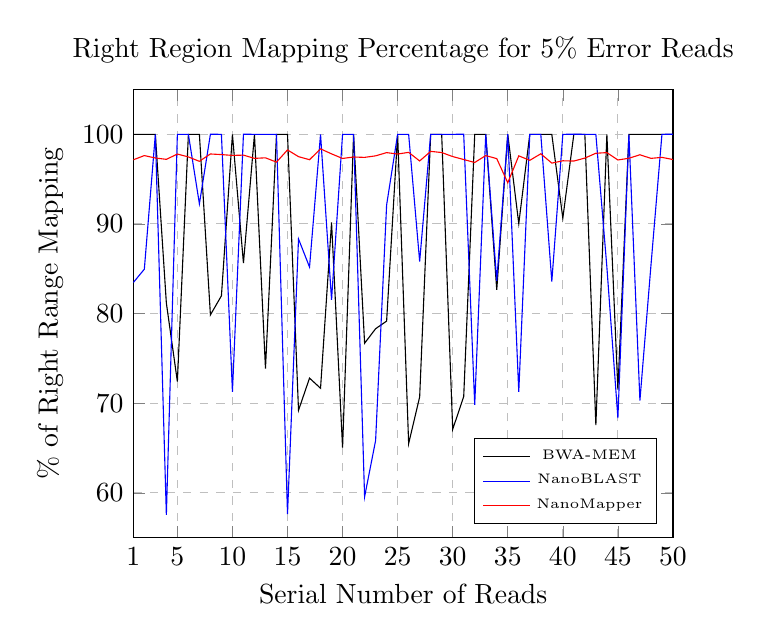
\begin{tikzpicture}
	\begin{axis}[
	title={Right Region Mapping Percentage for 5\% Error Reads},
	xlabel={Serial Number of Reads},
	ylabel={\% of Right Range Mapping  },
	xmin=1, xmax=50,
	ymin=55, ymax=105,
	xtick={1,5,10,15,20,25,30,35,40,45,50},
	ytick={60,70,80,90,100},
	legend pos=south east,
	legend style={font=\tiny},
	ymajorgrids=true,
	xmajorgrids=true,
	grid style=dashed,
	]
	
	\addplot[
	color=black,
	mark=dot,
	]
	coordinates {
		( 1 , 99.98 )( 2 , 99.98 )( 3 , 99.98 )( 4 , 81.17 )( 5 , 72.42 )( 6 , 99.98 )( 7 , 99.98 )( 8 , 79.85 )( 9 , 81.98 )( 10 , 99.98 )( 11 , 85.62 )( 12 , 99.98 )( 13 , 73.86 )( 14 , 99.98 )( 15 , 99.98 )( 16 , 69.21 )( 17 , 72.8 )( 18 , 71.67 )( 19 , 90.16 )( 20 , 65.04 )( 21 , 99.98 )( 22 , 76.69 )( 23 , 78.31 )( 24 , 79.16 )( 25 , 99.98 )( 26 , 65.5 )( 27 , 70.7 )( 28 , 99.98 )( 29 , 99.98 )( 30 , 67.09 )( 31 , 70.74 )( 32 , 99.98 )( 33 , 99.98 )( 34 , 82.64 )( 35 , 99.99 )( 36 , 90.03 )( 37 , 99.99 )( 38 , 99.98 )( 39 , 99.98 )( 40 , 90.64 )( 41 , 99.99 )( 42 , 99.98 )( 43 , 67.56 )( 44 , 99.98 )( 45 , 71.52 )( 46 , 99.98 )( 47 , 99.98 )( 48 , 99.98 )( 49 , 99.98 )( 50 , 99.98 )
	};
	\addlegendentry{BWA-MEM}
	\addplot[
	color=blue,
	mark=dot,
	]
	coordinates {
		( 1 , 83.46 )( 2 , 84.95 )( 3 , 99.99 )( 4 , 57.55 )( 5 , 99.99 )( 6 , 99.99 )( 7 , 92.24 )( 8 , 100.0 )( 9 , 99.99 )( 10 , 71.28 )( 11 , 100.0 )( 12 , 99.99 )( 13 , 99.99 )( 14 , 99.99 )( 15 , 57.63 )( 16 , 88.32 )( 17 , 85.19 )( 18 , 99.99 )( 19 , 81.53 )( 20 , 99.99 )( 21 , 99.99 )( 22 , 59.56 )( 23 , 65.84 )( 24 , 92.11 )( 25 , 99.99 )( 26 , 99.99 )( 27 , 85.81 )( 28 , 99.99 )( 29 , 99.99 )( 30 , 99.99 )( 31 , 100.0 )( 32 , 69.82 )( 33 , 99.99 )( 34 , 83.66 )( 35 , 100.0 )( 36 , 71.27 )( 37 , 99.99 )( 38 , 99.99 )( 39 , 83.58 )( 40 , 99.99 )( 41 , 100.0 )( 42 , 99.99 )( 43 , 99.98 )( 44 , 85.18 )( 45 , 68.35 )( 46 , 99.99 )( 47 , 70.3 )( 48 , 85.34 )( 49 , 99.99 )( 50 , 100.0 )
	};
	\addlegendentry{NanoBLAST}
	\addplot[
	color=red,
	mark=dot,
	]
	coordinates {
		( 1 , 97.15 )( 2 , 97.62 )( 3 , 97.35 )( 4 , 97.2 )( 5 , 97.79 )( 6 , 97.47 )( 7 , 96.98 )( 8 , 97.8 )( 9 , 97.73 )( 10 , 97.64 )( 11 , 97.67 )( 12 , 97.31 )( 13 , 97.37 )( 14 , 96.89 )( 15 , 98.25 )( 16 , 97.5 )( 17 , 97.16 )( 18 , 98.37 )( 19 , 97.81 )( 20 , 97.3 )( 21 , 97.46 )( 22 , 97.42 )( 23 , 97.59 )( 24 , 97.95 )( 25 , 97.79 )( 26 , 97.98 )( 27 , 97.02 )( 28 , 98.09 )( 29 , 97.96 )( 30 , 97.51 )( 31 , 97.18 )( 32 , 96.85 )( 33 , 97.62 )( 34 , 97.28 )( 35 , 94.59 )( 36 , 97.59 )( 37 , 97.09 )( 38 , 97.82 )( 39 , 96.78 )( 40 , 97.04 )( 41 , 97.01 )( 42 , 97.34 )( 43 , 97.88 )( 44 , 97.95 )( 45 , 97.13 )( 46 , 97.32 )( 47 , 97.71 )( 48 , 97.31 )( 49 , 97.42 )( 50 , 97.18 )
	};
	\addlegendentry{NanoMapper}
	\end{axis}
	\end{tikzpicture}
	
	
	\caption{Percentage of Right Range Mapping Comparison Among Tools.} \label{fig:mapComp}
\end{figure}

If we just eliminate mapping length less than or equal to 15, the accuracy reaches 99.17\%. In fact, these should be eliminated as these are not our target K-mer. We are mapping based on long K-mers. However, from figure \ref{fig:mapComp}, it is clear that NanoMapper always maintaining a consistant accuracy where other tools are showing curly curves. The consistent line drift upward when we eliminate K-mers less than or equal to length 15.

\begin{figure}
	\centering
	
	
	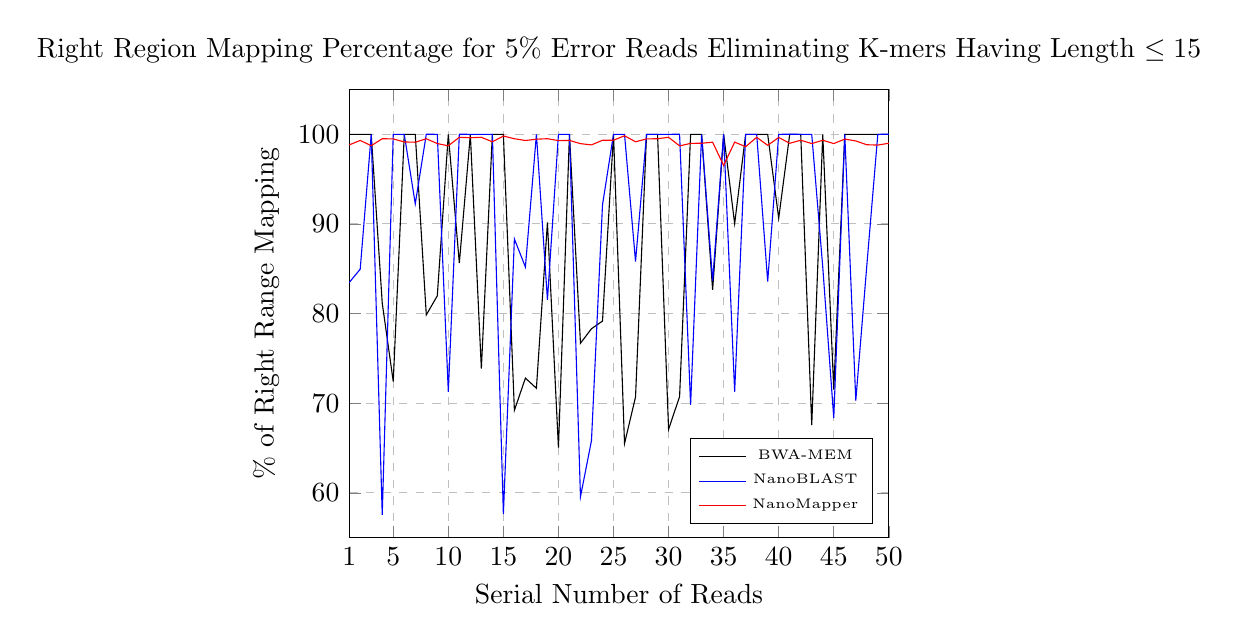
\begin{tikzpicture}
	\begin{axis}[
	title={Right Region Mapping Percentage for 5\% Error Reads Eliminating K-mers Having Length $\leq 15$},
	xlabel={Serial Number of Reads},
	ylabel={\% of Right Range Mapping  },
	xmin=1, xmax=50,
	ymin=55, ymax=105,
	xtick={1,5,10,15,20,25,30,35,40,45,50},
	ytick={60,70,80,90,100},
	legend pos=south east,
	legend style={font=\tiny},
	ymajorgrids=true,
	xmajorgrids=true,
	grid style=dashed,
	]
	
	\addplot[
	color=black,
	mark=dot,
	]
	coordinates {
		( 1 , 99.98 )( 2 , 99.98 )( 3 , 99.98 )( 4 , 81.17 )( 5 , 72.42 )( 6 , 99.98 )( 7 , 99.98 )( 8 , 79.85 )( 9 , 81.98 )( 10 , 99.98 )( 11 , 85.62 )( 12 , 99.98 )( 13 , 73.86 )( 14 , 99.98 )( 15 , 99.98 )( 16 , 69.21 )( 17 , 72.8 )( 18 , 71.67 )( 19 , 90.16 )( 20 , 65.04 )( 21 , 99.98 )( 22 , 76.69 )( 23 , 78.31 )( 24 , 79.16 )( 25 , 99.98 )( 26 , 65.5 )( 27 , 70.7 )( 28 , 99.98 )( 29 , 99.98 )( 30 , 67.09 )( 31 , 70.74 )( 32 , 99.98 )( 33 , 99.98 )( 34 , 82.64 )( 35 , 99.99 )( 36 , 90.03 )( 37 , 99.99 )( 38 , 99.98 )( 39 , 99.98 )( 40 , 90.64 )( 41 , 99.99 )( 42 , 99.98 )( 43 , 67.56 )( 44 , 99.98 )( 45 , 71.52 )( 46 , 99.98 )( 47 , 99.98 )( 48 , 99.98 )( 49 , 99.98 )( 50 , 99.98 )
	};
	\addlegendentry{BWA-MEM}
	\addplot[
	color=blue,
	mark=dot,
	]
	coordinates {
		( 1 , 83.46 )( 2 , 84.95 )( 3 , 99.99 )( 4 , 57.55 )( 5 , 99.99 )( 6 , 99.99 )( 7 , 92.24 )( 8 , 100.0 )( 9 , 99.99 )( 10 , 71.28 )( 11 , 100.0 )( 12 , 99.99 )( 13 , 99.99 )( 14 , 99.99 )( 15 , 57.63 )( 16 , 88.32 )( 17 , 85.19 )( 18 , 99.99 )( 19 , 81.53 )( 20 , 99.99 )( 21 , 99.99 )( 22 , 59.56 )( 23 , 65.84 )( 24 , 92.11 )( 25 , 99.99 )( 26 , 99.99 )( 27 , 85.81 )( 28 , 99.99 )( 29 , 99.99 )( 30 , 99.99 )( 31 , 100.0 )( 32 , 69.82 )( 33 , 99.99 )( 34 , 83.66 )( 35 , 100.0 )( 36 , 71.27 )( 37 , 99.99 )( 38 , 99.99 )( 39 , 83.58 )( 40 , 99.99 )( 41 , 100.0 )( 42 , 99.99 )( 43 , 99.98 )( 44 , 85.18 )( 45 , 68.35 )( 46 , 99.99 )( 47 , 70.3 )( 48 , 85.34 )( 49 , 99.99 )( 50 , 100.0 )
	};
	\addlegendentry{NanoBLAST}
	\addplot[
	color=red,
	mark=dot,
	]
	coordinates {
		( 1 , 98.81 )( 2 , 99.31 )( 3 , 98.72 )( 4 , 99.5 )( 5 , 99.48 )( 6 , 99.14 )( 7 , 99.11 )( 8 , 99.5 )( 9 , 98.96 )( 10 , 98.71 )( 11 , 99.66 )( 12 , 99.61 )( 13 , 99.66 )( 14 , 99.16 )( 15 , 99.8 )( 16 , 99.5 )( 17 , 99.3 )( 18 , 99.45 )( 19 , 99.5 )( 20 , 99.29 )( 21 , 99.31 )( 22 , 98.95 )( 23 , 98.81 )( 24 , 99.33 )( 25 , 99.33 )( 26 , 99.83 )( 27 , 99.16 )( 28 , 99.48 )( 29 , 99.5 )( 30 , 99.66 )( 31 , 98.7 )( 32 , 98.98 )( 33 , 99.0 )( 34 , 99.11 )( 35 , 96.52 )( 36 , 99.12 )( 37 , 98.61 )( 38 , 99.66 )( 39 , 98.76 )( 40 , 99.64 )( 41 , 98.99 )( 42 , 99.33 )( 43 , 98.96 )( 44 , 99.33 )( 45 , 98.96 )( 46 , 99.46 )( 47 , 99.25 )( 48 , 98.83 )( 49 , 98.79 )( 50 , 99.0 )
	};
	\addlegendentry{NanoMapper}
	\end{axis}
	\end{tikzpicture}
\caption{Percentage of Right Range Mapping Comparison Among Tools After Removing K-mer Having Length Less Than or Equal to 15.} \label{fig:mapComp1}
\end{figure}

\begin{table}[]
	\centering
	\caption{Mapping Comparison While 10\% Error Added in Read Data Eliminating K-mer Having Length $\leq 15$.}
	\label{tab:error10}
	\begin{tabular}{|c|c|c|}
		\hline
		\begin{tabular}[c]{@{}c@{}}Name of the\\ Tool\end{tabular} & \begin{tabular}[c]{@{}c@{}}Right Position\\ (\%)\end{tabular} & \begin{tabular}[c]{@{}c@{}}Wrong Position\\ (\%)\end{tabular} \\ \hline
		BWA-MEM & 88.82 & 11.18 \\ \hline
		NanoBLAST & 88.72 & 11.28 \\ \hline
		NanoMapper & 99.02 & 0.98 \\ \hline
	\end{tabular}
\end{table}

When 10\% error added in the read, the performance of NanoBLAST became a little bit better than before. Table \ref{tab:error10} shows that With removing K-mers $\leq 15$, NanoMapper still outperforming any other existing tools. From the figure \ref{fig:mapComp2}, it could be noticed that for the read \#15, NanoMapper's consistency degraded. But for that case, both the other tools give worse performance.

\begin{figure}
	\centering
	
	
	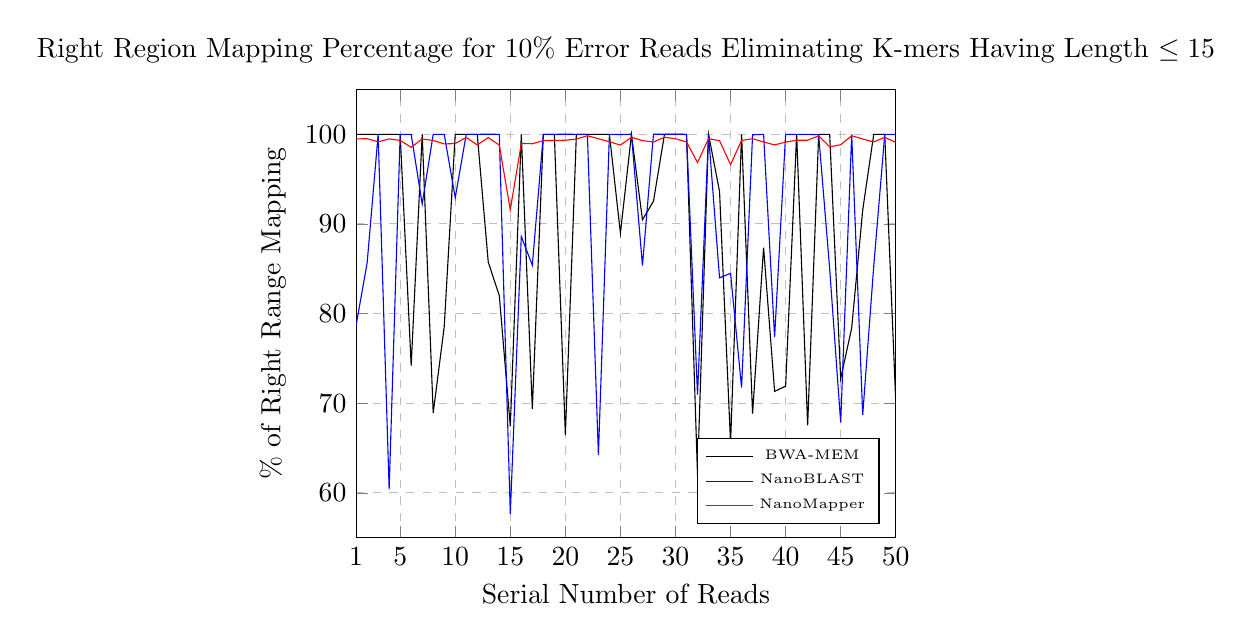
\begin{tikzpicture}
	\begin{axis}[
	title={Right Region Mapping Percentage for 10\% Error Reads Eliminating K-mers Having Length $\leq 15$},
	xlabel={Serial Number of Reads},
	ylabel={\% of Right Range Mapping  },
	xmin=1, xmax=50,
	ymin=55, ymax=105,
	xtick={1,5,10,15,20,25,30,35,40,45,50},
	ytick={60,70,80,90,100},
	legend pos=south east,
	legend style={font=\tiny},
	ymajorgrids=true,
	xmajorgrids=true,
	grid style=dashed,
	]
	
	\addplot[
	color=black,
	mark=dot,
	]
	coordinates {
		( 1 , 99.99 )( 2 , 99.98 )( 3 , 99.98 )( 4 , 99.98 )( 5 , 99.99 )( 6 , 74.19 )( 7 , 99.99 )( 8 , 68.91 )( 9 , 78.53 )( 10 , 99.99 )( 11 , 99.98 )( 12 , 99.98 )( 13 , 85.72 )( 14 , 82.02 )( 15 , 67.43 )( 16 , 99.98 )( 17 , 69.37 )( 18 , 99.98 )( 19 , 99.98 )( 20 , 66.45 )( 21 , 99.98 )( 22 , 99.98 )( 23 , 99.98 )( 24 , 99.98 )( 25 , 88.95 )( 26 , 99.98 )( 27 , 90.46 )( 28 , 92.53 )( 29 , 99.98 )( 30 , 99.98 )( 31 , 99.99 )( 32 , 61.98 )( 33 , 99.99 )( 34 , 93.61 )( 35 , 65.55 )( 36 , 99.98 )( 37 , 68.83 )( 38 , 87.36 )( 39 , 71.32 )( 40 , 71.9 )( 41 , 99.98 )( 42 , 67.52 )( 43 , 99.98 )( 44 , 99.99 )( 45 , 72.76 )( 46 , 78.4 )( 47 , 91.54 )( 48 , 99.98 )( 49 , 99.99 )( 50 , 70.14 )
	};
	\addlegendentry{BWA-MEM}
	\addplot[
	color=blue,
	mark=dot,
	]
	coordinates {
		( 1 , 78.7 )( 2 , 85.64 )( 3 , 99.99 )( 4 , 60.4 )( 5 , 99.99 )( 6 , 99.99 )( 7 , 92.22 )( 8 , 99.99 )( 9 , 99.99 )( 10 , 92.93 )( 11 , 99.99 )( 12 , 99.99 )( 13 , 100.0 )( 14 , 99.99 )( 15 , 57.67 )( 16 , 88.6 )( 17 , 85.39 )( 18 , 99.99 )( 19 , 99.99 )( 20 , 100.0 )( 21 , 99.99 )( 22 , 99.99 )( 23 , 64.24 )( 24 , 99.99 )( 25 , 99.97 )( 26 , 100.0 )( 27 , 85.34 )( 28 , 100.0 )( 29 , 100.0 )( 30 , 100.0 )( 31 , 99.99 )( 32 , 70.96 )( 33 , 99.99 )( 34 , 83.98 )( 35 , 84.5 )( 36 , 71.74 )( 37 , 99.94 )( 38 , 99.99 )( 39 , 77.37 )( 40 , 99.99 )( 41 , 99.99 )( 42 , 99.99 )( 43 , 99.95 )( 44 , 84.98 )( 45 , 67.84 )( 46 , 99.98 )( 47 , 68.7 )( 48 , 85.26 )( 49 , 99.99 )( 50 , 99.99 )
	};
	\addlegendentry{NanoBLAST}
	\addplot[
	color=red,
	mark=dot,
	]
	coordinates {
		( 1 , 99.48 )( 2 , 99.5 )( 3 , 99.16 )( 4 , 99.48 )( 5 , 99.31 )( 6 , 98.54 )( 7 , 99.47 )( 8 , 99.31 )( 9 , 98.92 )( 10 , 98.96 )( 11 , 99.64 )( 12 , 98.81 )( 13 , 99.63 )( 14 , 98.79 )( 15 , 91.57 )( 16 , 98.98 )( 17 , 98.94 )( 18 , 99.29 )( 19 , 99.31 )( 20 , 99.33 )( 21 , 99.47 )( 22 , 99.83 )( 23 , 99.5 )( 24 , 99.16 )( 25 , 98.79 )( 26 , 99.66 )( 27 , 99.29 )( 28 , 99.14 )( 29 , 99.66 )( 30 , 99.5 )( 31 , 99.14 )( 32 , 96.85 )( 33 , 99.5 )( 34 , 99.28 )( 35 , 96.61 )( 36 , 99.31 )( 37 , 99.5 )( 38 , 99.14 )( 39 , 98.81 )( 40 , 99.12 )( 41 , 99.33 )( 42 , 99.33 )( 43 , 99.83 )( 44 , 98.6 )( 45 , 98.83 )( 46 , 99.83 )( 47 , 99.47 )( 48 , 99.14 )( 49 , 99.66 )( 50 , 99.09 )
	};
	\addlegendentry{NanoMapper}
	\end{axis}
	\end{tikzpicture}
	\caption{Percentage of Right Range Mapping Comparison Among Tools After Removing K-mer Having Length Less Than or Equal to 15 For 10\% Noise In Data.} \label{fig:mapComp2}
\end{figure}

\end{document}
%\documentclass{standalone}
\usepackage{standalone}

\begin{document}
\chapter{Conclusion}
The remarkable notes are briefed below. Another section describe how the tool could be made more useful for the world and could be served in greater extent.
\section{Discussion}
NanoBASTer\cite{nanoBLAST} of Mohammad Ruhul Amin, BWA\cite{BWA_short} and BWA-SW\cite{BWA_long} of Heng Li, Bowtie\cite{bowtie} and Bowtie2\cite{bowtie2} of Ben Langmead are good alignment tools. But none of them could be selected and announced as the best to use in general. Minimap\cite{minimap} of Heng Li also a recent tool which is developed for mainly assembly tool like miniasm\cite{minimap} of him. From their work, we learnt a lot of thing. Before this, the concept of Minimizer\cite{KMC2,KMC}, Bloom filter\cite{BFCounter,turtle}, Hash Table\cite{corman,jellyfish}, Count-min Sketch\cite{minsketch}, Locality Sensitive Hashing\cite{LSH} etc. helped us a lot to think from different perspective.
\end{document}
%\documentclass{standalone}
\usepackage{standalone}

\begin{document}
\section{Future Work}
\subsection{API Enhancement}
Our used API for FM-index, SDSL-lite\cite{SDSL}, is not that fast comparing with other existing tools. This implementation is a general purpose API. So, tweaking for only four letter in the alphabet could be done.
\subsection{Integration with NanoBLASTer}
One of the drawbacks of NanoBLASTer\cite{nanoBLAST} is it could not recognize long insertion or long deletion. So, it is the best implementation to enhance the performance and reduce the problem. As the input output format and parameters in functions disagree between NanoBLASTer and this tool, the integration has not been done. With some effort, it could be done easily to get output in greater extent.
\subsection{Testing}
As our datasets and resources were limited we could not test the tool vastly. Massive testing would build a set of statistics based on which some heuristics might be added to get better output. 
\subsection{Developing New Aligner}
Based on this mapping tool, a new aligner tool could be made for some specific project. This may take lot of time to build such one, but it would be effective if built once. Enhanced alignment like Gotoh\cite{gotoh,gotoh1} and other could be developed and run parallel to this which may give a good output.
\par 
Currently this tool generates some  
\begin{verbatim}
<variable_length_kmer>  <pos_in_read>  <pos_in_reference>
\end{verbatim}
triplets for each read. Then to map the whole read to the desired segment of the reference we would need to cluster the triplets such that the maximum cluster will be formed with the maximum count of minimizers that maintains order both in read and reference.
\par 
Many type of clustering technique has been used in different tools. For example Miniasm-Minimap\cite{minimap} uses a clustering technique that is inspired from Hough Transformation\cite{HT1, HT2} a feature extraction technique used in Digital image processing, MUMmer uses their own clustering technique.	  
\end{document}

\clearpage
\renewcommand\bibname{References}
\bibliographystyle{IEEEtran}
\bibliography{IEEEabrv,references}

\begin{appendices}
	%\documentclass{standalone}
\usepackage{standalone}

\begin{document}
	\chapter{Setting Up NanoMapper}
	A unix based operating system is needed to run this program. Please ensure that the system fulfilled the following requirements:
	\begin{itemize}
		\item The latest version of of C++ compiler. C++11 standard or later. clang version must be 3.2 or higher.
		\item A cmake build system.
		\item The operating system must be a 64-bit machine.
		\item zlib library installed.
	\end{itemize}
	\section{API}
	The SDSL-lite\cite{SDSL} API is used to implement FM-index. It could be installed by the following command lines in the terminal:
	\begin{verbatim}
	    $ git clone https://github.com/simongog/sdsl-lite.git
	    $ cd sdsl-lite
	    $ ./install.sh
	\end{verbatim}
	The API could be un-installed after working by the following command having same directory in the terminal:
	\begin{verbatim}
	    $ ./uninstall.sh
	\end{verbatim}
	\section{Installing NanoMapper}
	The following commands in terminal would let you install NanoMapper in your PC:
	\begin{verbatim}
	    $ git clone https://github.com/enamcse/NanoMapper.git && cd NanoMapper
	    $ g++ -o NanoMapper -std=c++11 -O3 -DNDEBUG -I ~/include -L ~/lib 
	      Main_minimizer.cpp -lz -lsdsl -ldivsufsort -ldivsufsort64
	\end{verbatim}
	\section{Running NanoMapper}
	The NanoMapper could be run on your PC giving the parameters like below:
	\begin{verbatim}
	    $ ./NanoMapper <path_of_reference_file> <path_of_reads_file> 
	      <K-mer_length> <window_length> 
	      <output_file_path_for_naive_fm_index_approach>
	      <output_file_path_for_enhanced_fm_index_approach>
	\end{verbatim}
	Example:
	\begin{verbatim}
	    $ ./NanoMapper synthetic_reference_seq.fasta gen_seq.fasta 14 24 
	      loc_syn_out.txt loc_syn_out_1.txt
	\end{verbatim}
	Note that, each command should be given in one line. Here, it is shown in multi-line for simplicity.
\end{document}
\end{appendices}

\end{document}